\documentclass[11pt, openright]{book}

    % Cover Variables
    \newcommand{\ctitle}{Title}
    \newcommand{\cautor}{Author}
    \newcommand{\ctoptitle}{}

    % Header Variables
    
        \newcommand{\headRE}{\emph{\thesection. \leftmark}}
        \newcommand{\headLE}{\emph{\thepage}}
        \newcommand{\footRE}{}
        \newcommand{\footLE}{\text{\rightmark}}

    % TOC Variables
        \newcommand{\toctitle}{Table of Content}
        \newcommand{\tocchapter}{Chapter}
        \newcommand{\toccount}{3}
  
    % Chapter Variables
        \newcommand{\chvar}{Chapter -}




% Page Style
\usepackage[]{environ}
% Cover Page 
\usepackage{tikz}
\makeatletter
\def\parsecomma#1,#2\endparsecomma{\def\page@x{#1}\def\page@y{#2}}
\tikzdeclarecoordinatesystem{page}{
    \parsecomma#1\endparsecomma
    \pgfpointanchor{current page}{north east}
    % Save the upper right corner
    \pgf@xc=\pgf@x%
    \pgf@yc=\pgf@y%
    % save the lower left corner
    \pgfpointanchor{current page}{south west}
    \pgf@xb=\pgf@x%
    \pgf@yb=\pgf@y%
    % Transform to the correct placement
    \pgfmathparse{(\pgf@xc-\pgf@xb)/2.*\page@x+(\pgf@xc+\pgf@xb)/2.}
    \expandafter\pgf@x\expandafter=\pgfmathresult pt
    \pgfmathparse{(\pgf@yc-\pgf@yb)/2.*\page@y+(\pgf@yc+\pgf@yb)/2.}
    \expandafter\pgf@y\expandafter=\pgfmathresult pt
}
\makeatother


% Object formatting
\usepackage[12pt]{moresize}
\usepackage[]{anyfontsize}
\usepackage{titlesec}
\usepackage{import}
\usepackage{floatrow}
\usepackage{enumitem}
\usepackage{changepage}
\usepackage[normalem]{ulem}
\usepackage{array}
\newcommand{\ul}[1]{\underline{#1}}

\usepackage[]{chngcntr}
\counterwithin{figure}{section}
\usepackage[format=plain, labelfont=it, textfont=it]{caption}
\makeatletter
\def\@makecaption#1#2{%
    \vskip\abovecaptionskip
    \sbox\@tempboxa{\textit{\thearsection.\thefigure. #2}}
    \ifdim \wd\@tempboxa >\hsize
        #1. #2\par
    \else
        \global \@minipagefalse
        \hb@xt@\hsize{\hfil\box\@tempboxa\hfil}
    \fi
    \vskip\belowcaptionskip}
\makeatother

\DeclareCaptionFormat{underline}{\uline{#1#2#3}\par}

% Sections
\titleformat{\section}{\fontsize{15}{18}\bfseries}{Lesson \thesection.}{0.25em}{}
\titleformat{\subsection}{\fontsize{14}{16.8}\bfseries}{\tab}{0.25em}{}
\titleformat{\subsubsection}{\fontsize{10}{12}}{\uline{\thesubsubsection)\enspace}}{0em}{\uline}





% Geometry
\usepackage{fancyhdr}
\usepackage{ragged2e}
\usepackage[a4paper, total={18.625cm, 22.125cm}]{geometry}

% Typewriting

\setlength{\parskip}{1em}
\setlength{\parindent}{0em}

% List Formatting
\NewEnviron{items}[3][0pt]{
    \vspace{#2}
    \begin{itemize}
        \setlength{\itemsep}{#1}
        \setlength{\topsep}{0pt}
        \setlength{\partopsep}{0pt}
        \BODY
    \end{itemize}\vspace{#3}}

\NewEnviron{enum}[3][0pt]{%
    \vspace{#2}%
    \begin{enumerate}%
        \setlength{\itemsep}{#1}%
        \setlength{\topsep}{0pt}%
        \setlength{\partopsep}{0pt}%
        \BODY
    \end{enumerate}
    \vspace{#3}}%

\NewEnviron{eq}[2]{%
    \vspace{#1}%
    \begin{align*}%
        \BODY
    \end{align*}
    \vspace{#2}}%

\NewEnviron{dent}[1]{
    \begin{adjustwidth}{7mm}{}
        \uline{#1}\hspace{2mm}
        \BODY
    \end{adjustwidth}
}
\NewEnviron{lfeq}[2]{%
    \vspace{#1}%
    \begin{flalign*}%
        \BODY
    \end{flalign*}
    \vspace{#2}}%


% Functions and Data Plotting
\usepackage{subfig,wrapfig,adjustbox,multirow}


% Plotting Style
\usepackage{graphicx,pgfplots}
\usetikzlibrary{arrows.meta}
\usetikzlibrary {patterns,patterns.meta}
\usepgfplotslibrary{fillbetween}
\pgfplotsset{compat=1.18}

\usepgfplotslibrary{units}
% Logarithmic Scale
\pgfplotsset{
    log x ticks with fixed point/.style={
            xticklabel={
                    \pgfkeys{/pgf/fpu=true}
                    \pgfmathparse{exp(\tick)}%
                    \pgfmathprintnumber[fixed relative, precision=3]{\pgfmathresult}
                    \pgfkeys{/pgf/fpu=false}
                }
        }
}

% Mathematics

% Formatting
\usepackage{amsmath}
\usepackage{esvect}
\usepackage{amsfonts}
\usepackage{tasks,environ}
\usepackage{xargs}
\usepackage{esint}
\usepackage[]{listings}


\usepackage[english]{babel}
\usepackage{amsthm}
%\newtheorem{theorem}{Theorem}
%\newtheorem{proof}{Proof}



%Custom Shortcuts
\newcommand{\eqi}{\Leftrightarrow}
\newcommand{\lr}[1]{\left( #1 \right)}
\newcommand{\limit}[1]{\displaystyle{\lim_{#1}}}
\newcommand{\tab}{\hspace*{7mm}}
\newcommand{\ds}[1]{\displaystyle{#1}}
\newcommand{\floor}[1]{\lfloor #1 \rfloor}
\newcommand{\R}{\mathbb{R}}
\newcommand{\N}{\mathbb{N}}
\newcommand{\Z}{\mathbb{Z}}
\newcommand{\C}{\mathbb{C}}
\newcommand{\K}{\mathbb{K}}
\newcommand{\F}{\mathcal{F}}
\newcommand{\M}{\mathcal{M}}
\renewcommand{\l}{\lambda}
\newcommand{\seg}[1]{\overline{\rm {#1}}}
\newcommand{\Int}{\int\limits}
\newcommand{\ex}{\tab \uline{Example :}\hspace{0.2cm} }
\newcommand{\vard}{\partial}
\newcommand{\Q}{\mathcal{Q}}
\newcommand{\Vect}{\operatorname{Vect}}
\newcommand{\rg}{\operatorname{rg}}
\renewcommand{\dim}{\operatorname{dim}}
\renewcommand{\Re}{\operatorname{Re}}
\renewcommand{\Im}{\operatorname{Im}}
\renewcommand{\P}{\mathcal{P}}
\newcommand{\blr}[1]{\left\{#1\right\}}
\newcommand{\linecenter}[1]{\par\vspace{2mm} \centerline{#1}\par\vspace{-2mm}}
\newcommand{\dd}{\textrm{d}}
\newcommand{\supp}{\operatorname{Supp}}
\renewcommand{\vec}{\overrightarrow}
\renewcommand{\epsilon}{\varepsilon}

% Matrix Configurations

\makeatletter
\renewcommand*\env@matrix[1][*\c@MaxMatrixCols c]{%
    \hskip -\arraycolsep
    \let\@ifnextchar\new@ifnextchar
    \array{#1}}
\makeatother


% Colors
\usepackage{xcolor}
\newcommand{\blu}{\color{blue}}
\newcommand{\Red}{\color{red}}
\newcommand{\blac}{\color{black}}

\newcommand{\red}[1]{\textcolor{red}{#1}}

\usepackage{xcolor,xspace}
\usepackage{breqn}


% Headings  
\usepackage[Glenn]{fncychap}
\ChNumVar{\fontsize{40}{42}}
\ChTitleVar{\Large\sc}
\ChNameVar{\Large \sc}
\setlength\headheight{14.5pt}
\renewcommand\FmN[1]{\chvar}





% Header & Footers
\renewcommand{\chaptermark}[1]{\markboth{#1}{#1}}
\renewcommand{\sectionmark}[1]{
    \markright{#1}
}
\pagestyle{fancy}
\fancyhf{}
\fancyhead[LE,RO]{\headLE}
\fancyhead[RE,LO]{\headRE}
\fancyfoot[LE, RO]{\footLE}
\fancyfoot[LO, RE]{\footRE}
\renewcommand{\headrulewidth}{0.5pt}


\fancypagestyle{plain}{%
    \fancyhf{} % clear all header and footer fields
    \fancyfoot[LE, RO]{}
    \renewcommand{\headrulewidth}{0pt}
    \renewcommand{\footrulewidth}{0pt}}

\fancypagestyle{nohead}{%
    \fancyhf{} % clear all header 
    \fancyfoot[LE, RO]{}
    \fancyfoot[LO, RE]{}}


\fancypagestyle{bib}{%
    \fancyhf{} % clear all header and footer fields
    \fancyhead[CE, CO]{}
    \fancyfoot[LE, RO]{\footLE}
    \fancyfoot[LO, RE]{Bibliographie}}


% Table of Contents

\renewcommand*\thechapter{\arabic{chapter}} %Usually Roman
\renewcommand*\thesection{\arabic{section}}
\newcommand*\thearsection{\arabic{subsection}}
\renewcommand*\thesubsubsection{\thesubsection.\alph{subsubsection}}
\renewcommand*\thefigure{\arabic{figure}}
\makeatletter
\@removefromreset{section}{chapter}
\makeatother


% Table of Contents

\usepackage{titletoc}
\usepackage{ erewhon,cabin}
\usepackage[linktoc=all]{hyperref}
\renewcommand*\contentsname{\centerline{\toctitle}}

\setcounter{secnumdepth}{3}
\setcounter{tocdepth}{\toccount}

\usepackage[subfigure]{tocloft}
\setlength\cftparskip{0pt}

\usepackage{etoolbox}
\makeatletter
\pretocmd{\chapter}{\addtocontents{toc}{\protect\addvspace{5\p@}}\thispagestyle{plain}}{}{}
\pretocmd{\section}{\addtocontents{toc}{\protect\addvspace{-10\p@}}}{}{}
\pretocmd{\subsection}{\addtocontents{toc}{\protect\addvspace{1\p@}}}{}{}
\makeatother


% Chapter Style
\titlecontents{chapter}
[7em]
{\bigskip}
{\bfseries\textsc\tocchapter~\textsc\thecontentslabel : \textsc}
{\hspace*{-5.5em}\textbf}
{\titlerule*[1pc]{ }}[\smallskip]

% Section Style
\titlecontents{section}
[3em] % i
{\bigskip\bfseries}
{\fontsize{11}{13.2}\bfseries\uline{Lesson \thecontentslabel.\enspace}\uline}
{\hspace*{-4em}\textbf}
{\hspace{-2mm}\titlerule*[0.5pc]{\uline{\hspace{2.115mm}}}\contentspage}

% Subsection Style
\titlecontents{subsection}
[5em] % i
{\smallskip\bfseries}
{\fontsize{10}{12}\bfseries\thecontentslabel.\enspace}
{\hspace*{-4em}}
{\titlerule*[0.5pc]{.}\contentspage}



% Subsubsection Style
\titlecontents{subsubsection}
[7em] % i
{\smallskip}
{\fontsize{10}{12}\thecontentslabel)\enspace}
{\hspace*{-4em}}
{\titlerule*[0.5pc]{.}\contentspage}










    % figure support
    \usepackage{import}
    \usepackage{xifthen}
    \pdfminorversion=7
    \usepackage{pdfpages}
    \usepackage{transparent}
    \newcommand{\incfig}[1]{%
            \def\svgwidth{\columnwidth}
            \import{./figures/}{#1.pdf_tex}
    }

    \pdfsuppresswarningpagegroup=1


    \setcounter{tocdepth}{1}
    \renewcommand*\thechapter{\Roman{chapter}}
    \renewcommand*\thesection{\Roman{section}}

    \hfuzz=100pt
    \vfuzz=100pt
    \hbadness=10000



\begin{document}
% Spacing
% Section Spacing
\titlespacing\section{0pt}{3pt plus 2pt minus 2pt}{6pt plus 2pt minus 1pt}
\titlespacing\subsection{0pt}{0pt plus 1pt minus 1pt}{0pt plus 3pt minus 1pt}
\titlespacing\subsubsection{0pt}{0pt plus 0pt minus 0pt}{0pt plus 2pt minus 0pt}

\usetikzlibrary{shadows}

\newgeometry{left=2.5cm, width=16cm, bottom=2.5cm, top=2.5cm}






% Cover
\begin{titlepage}
    \newgeometry{top=1cm, width=21cm, bottom=1cm}
    \begin{center}
        \tikz[remember picture,overlay] \node[opacity=0.3,inner sep=0pt, anchor=east] at (current page.east){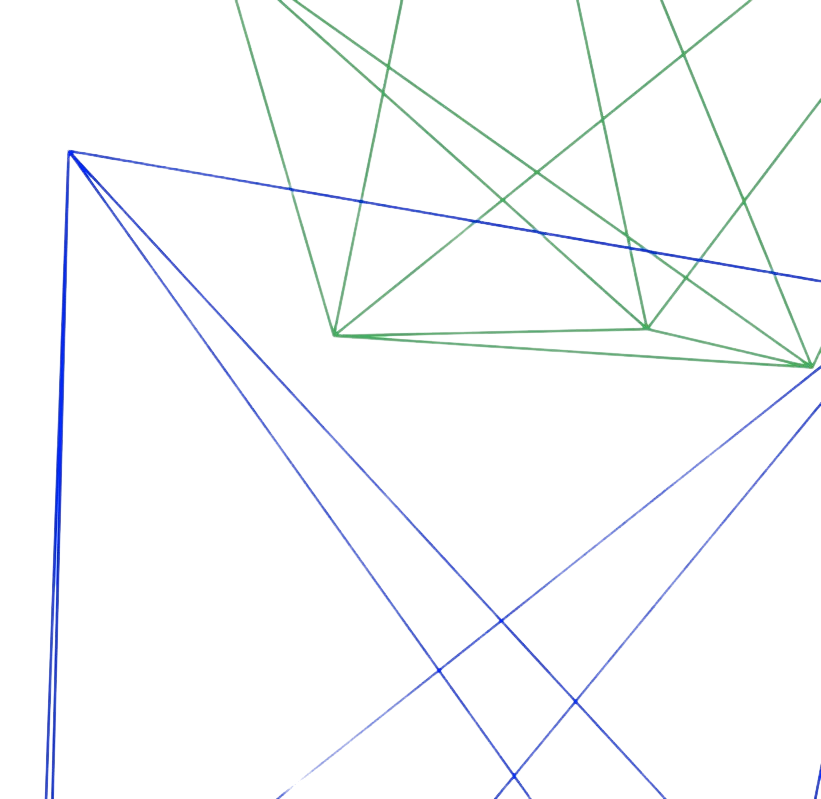
\includegraphics[width=0.5\paperwidth,height=\paperheight]{./logos/invert1.png}};
        \tikz[remember picture,overlay] \node[opacity=0.3,inner sep=0pt, anchor=south west] at (current page.south west){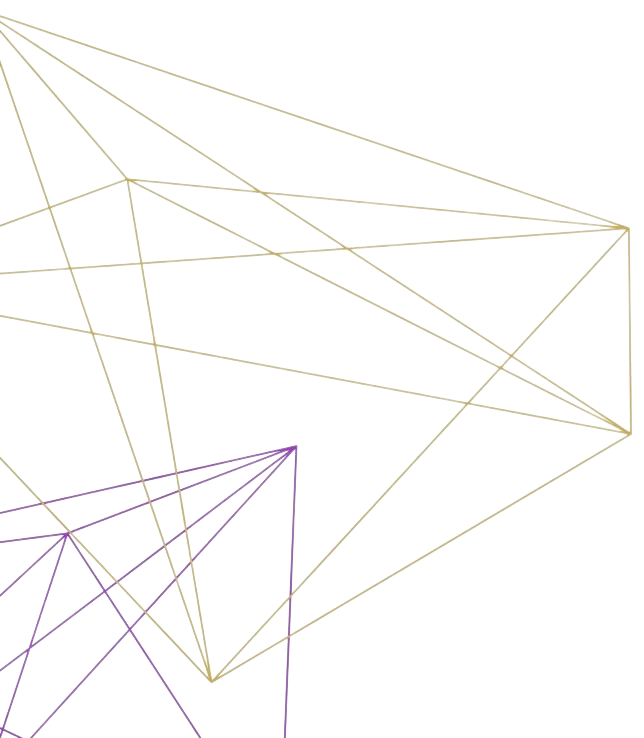
\includegraphics[width=0.5\paperwidth,height=0.5\paperheight]{./logos/invert2.png}};
        \tikz[remember picture,overlay] \node[opacity=0.3,inner sep=0pt, anchor=north west] at (current page.north west){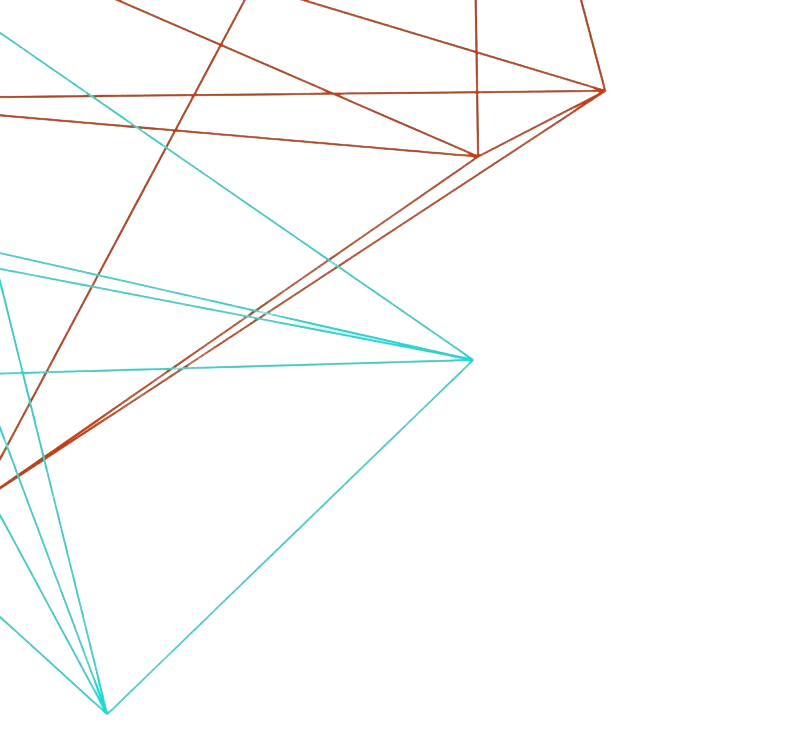
\includegraphics[width=0.5\paperwidth,height=0.5\paperheight]{./logos/invert3.png}};
    \end{center}


    \begin{tikzpicture}[remember picture,overlay,every node/.style={anchor=center}]
        \node (rectangle) at (page cs:0,0.4) [draw,thick, fill=white, minimum width=2cm,minimum height=2cm] {\HUGE\textbf{ DIFFERENTIAL EQUATIONS}};
    \end{tikzpicture}

    \begin{figure}[ht]
        
\includegraphics[height=1cm]{./logos/edx.png}
        \hspace{0.5cm}
        
\includegraphics[height=1cm]{./logos/Logo-W.jpg}
        \hspace{0.5cm}
        
\includegraphics[height=1cm]{./logos/OCW.png}
    \end{figure}

    \vspace{10cm}

    \begin{figure}[h]
        \centering
        
\includegraphics[width=0.5\textwidth]{./logos/Logo-old.png}
    \end{figure}
    \vspace{1cm}

\end{titlepage}
\newgeometry{width=18.625cm, bottom=2cm, top=2cm}

\tikz[remember picture, overlay] \node[opacity=0.3,inner sep=0pt, anchor=north east] at (current page.north east){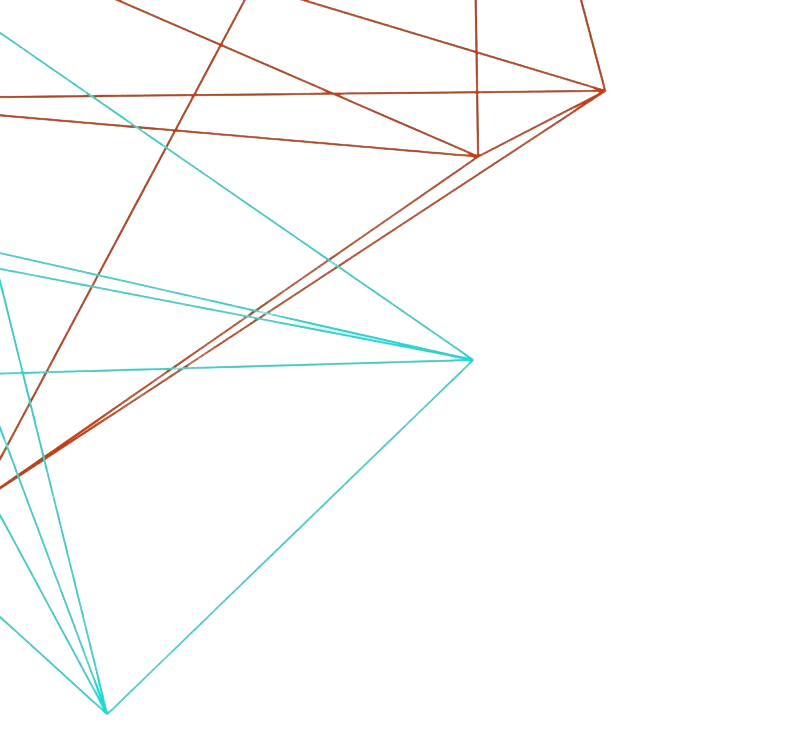
\includegraphics[angle=-90,origin=c,width=0.5\paperheight,height=0.5\paperwidth]{./logos/invert3.png}};
\tikz[remember picture,overlay] \node[opacity=0.3,inner sep=0pt, anchor=south east] at (current page.south east){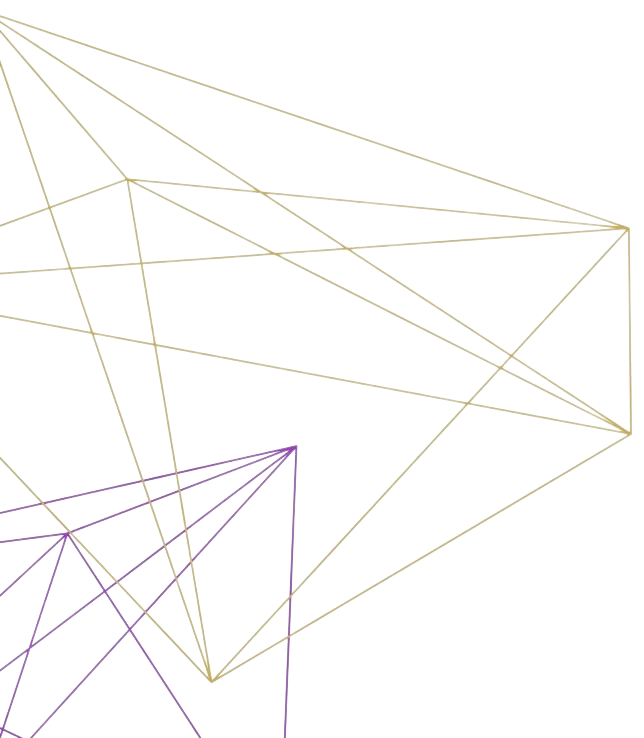
\includegraphics[angle=90,width=0.5\paperwidth,height=0.5\paperheight]{./logos/invert2.png}};

\thispagestyle{plain}
\newpage


\thispagestyle{fancy}
\tableofcontents


\newpage
\thispagestyle{plain}

\chapter{Modelling and First-Order Ordinary Differential Equations}

\section{Solving Simple Differential Equations and Modelling}

\subsection{Properties}

During the entirety of this course, we'll be going through different types of \red{Differential Equations}. First of which are the \red{Ordinary Differential Equations} where we often regard the independent variable to be time. ODEs always involve the derivatives of a function of only one variable. On the other end, we have \red{Partial Differential Equations} involving derivatives of a multivariable function.
\linecenter{Notation for higher derivatives of a function $\blu y(t)$ : $\ds{\blu y^{(n)}=\frac{d^ny}{dt^n}}$}
\begin{dent}{Example.}
    $\blu 9375\cos(t^5)\ddot{y}^4+982(y+t^2)^7\dot{y}-2ty^{(5)}=4087\sin(\frac{t}{y})+3786e^{y^3-t^2}+18.3$\\
    This equation is an ODE since it only involves derivatives with respect to one variable $\blu t$.

\end{dent}

Any linear ODE can be classified into 2 different types \red{homogeneous} and \red{inhomogeneous} linear ODE:
\begin{items}{-15pt}{-15pt}
    \item Homogeneous linear ODE is the same types of equations such as each summand is a function of $\blu t$, followed by any $n$-th order derivative:
    \linecenter{$\blu \ds{e^{t}\ddot{y}+5\dot{y}+t^3y=0}$\tab or \tab $\blu \ds{\mathcal{P}_{n}(t)y^{(n)}+\mathcal{P}_{n-1}(t)y^{(n-1)}+...+\mathcal{P}_0(t)y=0}$}
    \tab For some functions $\blu \mathcal{P}_{n}(t)\to\mathcal{P}_0(t)$ are called coefficients
    \item Inhomogeneous linear ODE are similar except that it has one term that is a function of $\blu t$ only, such as:
    \linecenter{$\blu \ds{e^{t}\ddot{y}+5\dot{y}+t^3y=\textcolor{red}{7\sin(t)}}$\tab or \tab $\blu \ds{\mathcal{P}_{n}(t)y^{(n)}+\mathcal{P}_{n-1}(t)y^{(n-1)}+...+\mathcal{P}_0(t)y=\color{red} q(t)}$}
\end{items}
Either of these two forms can be reduced further by dividing the entire differential equation by $\blu \mathcal{P}_n(t)$, this way the coefficient of the highest derivative becomes 1. A differential equation written in either of the forms where the leading coefficient is 1 is referred to as the \red{Standard Form}.

\note If $\blu y=0$ is a solution, the ODE is homogeneous else the ODE is inhomogeneous.

For an ODE to be non-linear the functions $\blu y$, $\blu \dot{y}$ must enter in a more complicated way: multiplied by each other, raised to the power, or with non-linear functions applied to them.
\linecenter{$\blu \ddot{y}-7ty\dot{y}=0\qquad \dot{y}=\cos(y+t)\qquad \dot{y}=y^2$}
Take the equations $\blu \dot{y}=ay$ and $\blu \dot{y}=-ay$, these would be classified as a \red{first-order linear homogeneous differential equation.}

\newpage

\subsection{Mathematical Modelling}


To convert real-world problems into mathematical equations we can follow the following guidelines:
\begin{items}{-10pt}{-10pt}
    \item Identify the relevant quantities, both knowns and unknowns and give them symbols
    \item Identify independent variables. The other quantities will be a function of them or constants. Often, time is the only variable.
    \item Write down equations expressing how the functions change in response to small changes in the independent variables. Also write any ``laws of nature'' relating the variables
\end{items}

Often simplifying assumptions need to be made; the challenge is to simplify the equation so that they can be solved, but so that they can still describe the real-world system well.



\begin{dent}{Example.}
    I have a savings account earning interest compounded daily, and I make frequent deposits or withdrawals into the account. Find an ODE with an initial condition to model the balance.

    \uline{Simplifying Assumptions}
    \begin{items}{-10pt}{-10pt}
        \item Daily compounding is almost the same as continuous compounding, so let's assume that interest is paid continuously instead of at the end of the day.
        \item Similarly let's assume that my deposit/withdrawals can be approximated by a continuous money flow at a certain rate, the set deposit rate.
    \end{items}

    \uline{Variables and Functions}
    \begin{items}{-15pt}{-10pt}
        \item $\blu P$ initial amount the account starts with
        \item $\blu t$ time from the start
        \item $\blu x$ balance
        \item $\blu I$ interest rate
        \item $\blu q$ net deposit rate
    \end{items}


    \uline{Equations :}\hspace{2mm} Now we want to decide how the balance changes as time changes. We'll estimate the change in the balance $\blu \Delta x$ as time increases from $\blu t$ to a time $\blu t+ \Delta t$. We can approximate the interest as:
    \linecenter{$\color{black}\textit{interest earned per dollar} \blu \approx I(t)\Delta t$}
    The balance in the account at time $\blu t$ is $\blu x(t)$. Therefore, the total interest earned from $\blu t$ to $\blu t+\Delta t$ is:
    \linecenter{$\color{black}\textit{total interest earned} \blu \approx I(t)x(t)\Delta t$}
    Meanwhile, money is put into the account at a rate of $q(t)$, so:
    \linecenter{$\color{black}\textit{net amount deposited}\blu \approx q(t)\Delta t$}
    Putting it all together, the change in balance is:
    \linecenter{$\blu \Delta x \approx I(t)x(t)\Delta t+q(t)\Delta t\quad \implies \quad \frac{\Delta x}{\Delta t} = I(t)x(t)+q(t)$}
    The smaller $\blu \Delta t$ is, the better the approximation becomes, and in the limit, as $\blu \Delta t \to 0$ we have:
    \linecenter{$\blu \frac{dx}{dt}=I(t)x(t)+q(t)$}
    Also we have an initial condition $\blu x(0)=P$ thus we can write the following ODE:
    \linecenter{$\blu \boxed{\dot{x}=I(t)x(t)+q(t), \quad x(0)=P}$}
\end{dent}

\newpage

\subsection{Systems and Signals}


Going back to our savings model, maybe for financial planning we're interested in testing different strategies (different functions of $q$) to see what balances $x$ they result in. To help with this we'll rewrite the ODE as: $\dot{x}-I(t)=q(t)$

In the ``system and signal'' language of engineering, $q$ is called the \red{input signal}, the bank is the \red{system}, and $x$ is the \red{output signal}. These terms do not have a mathematical meaning dictated by the differential equation alone; their interpretation is guided by the system being modeled. But the general picture is this:

\begin{figure}[ht]
    \centering
    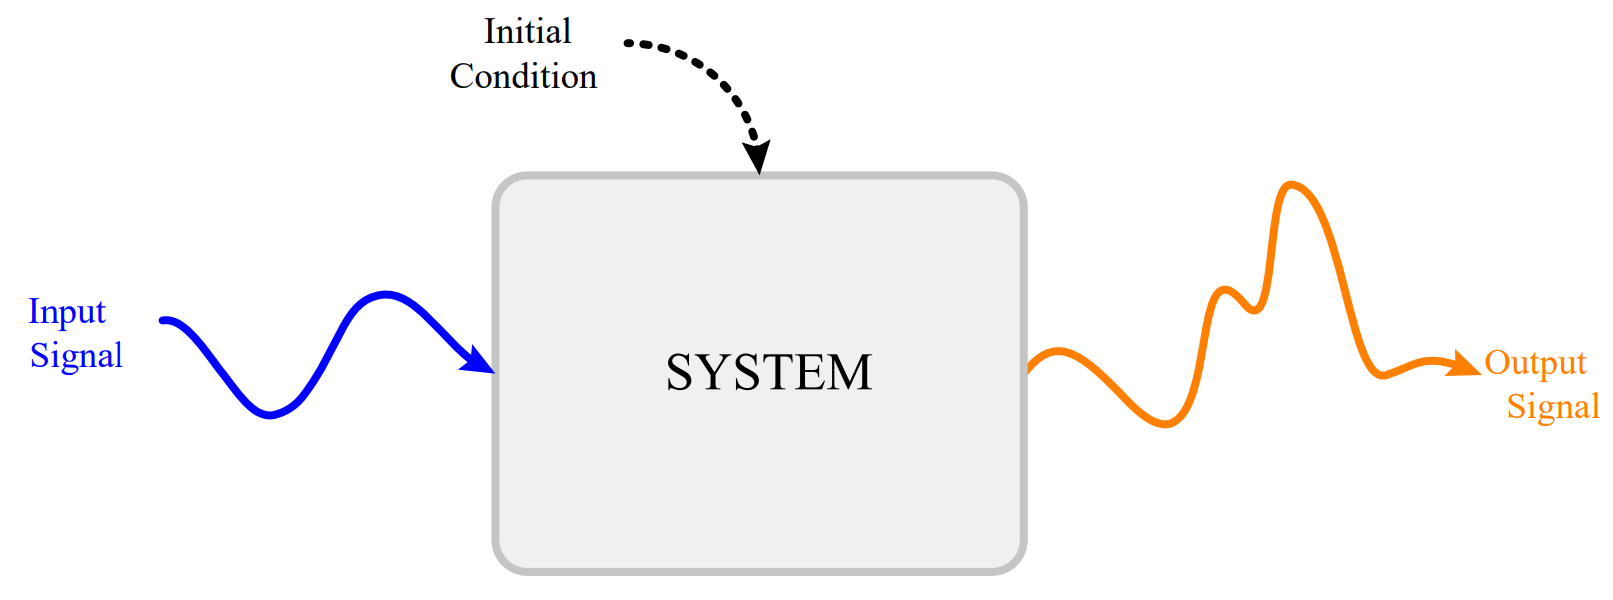
\includegraphics[width=0.7\textwidth]{./documents/l1/System.png}
\end{figure}

We'll see many of these modeled phenomena using this input system response language.

\begin{items}{-10pt}{-10pt}
    \item The \red{system} may be a mathematical application for a mechanical system such as a vehicle suspension or an electrical circuit. It is impacted by some external signal. We are interested in understanding how the system responds to the external signal.
    \item The \red{input signal} is the external stimulus. It usually does not appear simply in the differential equation as it does in the example alone. But it does always determine the right-hand side of the differential equation (when written in linear form).
    \item The \red{system response} (also called \red{output signal}) is the measurable behavior of the system that we are interested in. It is always the unknown function that we write a differential equation for.
\end{items}

All differential equations have many solutions. The solution of interest is often determined by the state of the system at the beginning. This initial state is given by the initial conditions.

\subsection{System using Newton's second law}


One of the most important sources for differential equations comes from Newton's second law: $\boxed{F=ma}$\\
Which is a differential equation written as $F=m\ddot{x}$

\begin{dent}{}
    Model a spring attached to a wall, with a mass on the other end sitting on a cart that moves without friction. We pull the cart back and release it. How does the mass on the cart behave?

    The variable of interest is the position of the mass, where $x$ is the displacement from the position when the spring is relaxed $x=0$, and $x>0$

    \begin{figure}[!htb]
        \floatsetup{floatrowsep=qquad}
        \begin{floatrow}
            \ffigbox[\FBwidth]{
                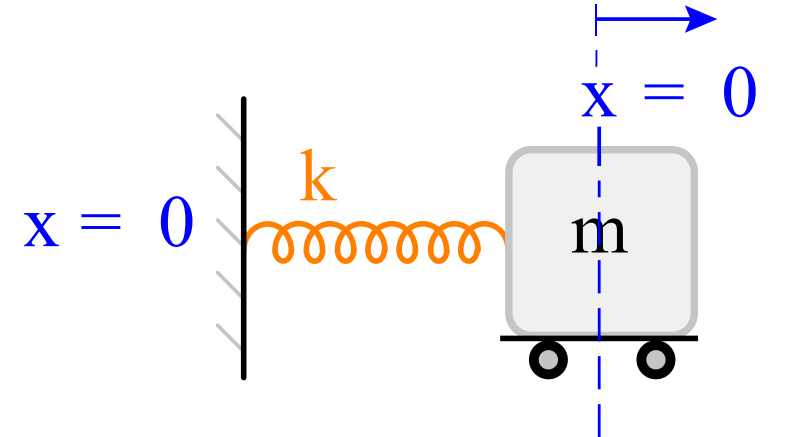
\includegraphics[height=0.1\textwidth]{./documents/l1/Relaxed.png}
                \caption{Relaxed}
            }

            \ffigbox[\FBwidth]{
                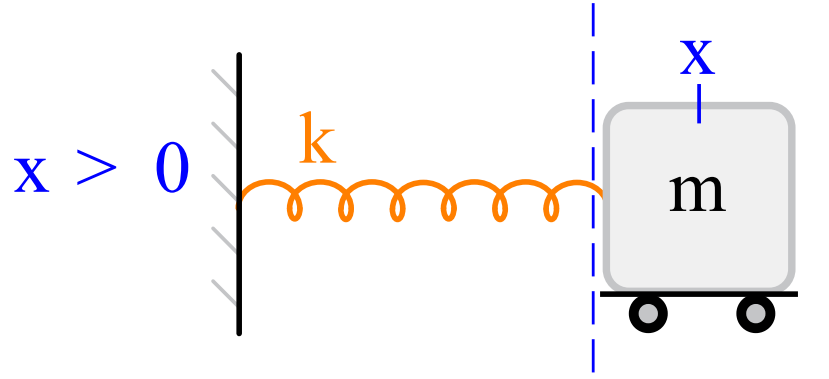
\includegraphics[height=0.1\textwidth]{./documents/l1/Stretched.png}
                \caption{Stretched}
            }

            \hspace{1.25cm}
            \ffigbox[\FBwidth]{
                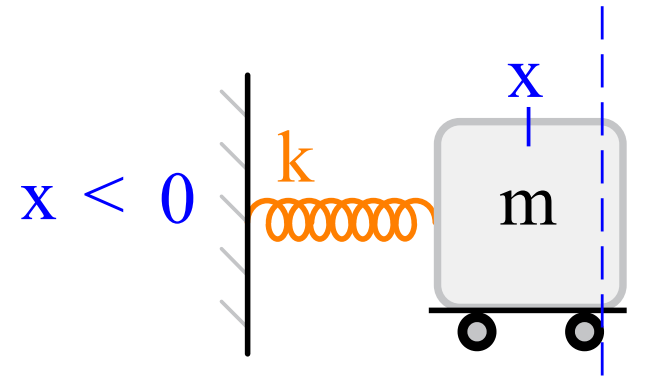
\includegraphics[height=0.1\textwidth]{./documents/l1/Compressed.png}
                \caption{Compressed}
            }

        \end{floatrow}
    \end{figure}

    \newpage

    Let's try to put this into the \red{input/system response} paradigm we've just introduced. The system response is the displacement of the mass

    What is the input signal? You could imagine other forces acting on the mass, such as wind blowing on a sail. But we are going to write down the differential equation governed by Newton's law: $F=m\ddot{x}$

    The only force acting on the mass is the spring force modeled linearly by Hooke's law: $F=-kx$

    Therefore we have $-kx=m\ddot{x}$ with initial conditions $x(0)=0$ and $\dot{x}(0)=0$

    The last step is to write this in standard linear form, we obtain the following differential equation:
    \linecenter{$\boxed{m\ddot{x}+kx=0\ \text{\textcolor{black}{with initial condition} }x(0)=x_0\ \text{\textcolor{black}{and }} \dot{x}(0)=0}$}
    In the case where the wind would've been an input signal, we would classify the differential equation $m\ddot{x}+kx=F_{wind}(t)$ as a second-order inhomogeneous differential equation.
\end{dent}

In the example above we've outlined 5 steps of our modeling process:
\begin{items}{-15pt}{-15pt}
    \item Draw a diagram of the system
    \item Identify and give symbols for the parameters and variables of the system
    \item Determine what is given or can be measured (could be the input signal) and what is to be determined (could be the system response). Identify any initial conditions
    \item Write down all equations relating the variables and parameters and manipulate them to join into a differential equation relating the chosen input signal and system response.
    \item If linear, rewrite the equation in standard linear form with initial conditions.
\end{items}

\newpage

\section{Solving First-2Order Ordinary Differential Equations}

\subsection{Separation of Variables}

Separation of variables is a technique that reduces the problem of solving certain first-order ODEs to evaluating two integrals, it works when we can write the equation in the form $\frac{dy}{dx}=g(t)f(y)$

\begin{dent}{}
    Solve $\dot{y}-2ty=0$

    \begin{items}{-15pt}{-15pt}
        \item Isolate the derivative and express in the form $\dot{y}=h(t,y)\ \implies\ \dot{y}=2ty$
        \item Write as $\frac{dy}{dx}=g(t)f(y)\ \implies\ g(t)=2t, f(y)=y$
        \item Separation, put the term involving $y$ on the left and the term involving $t$ on the right:\\
        \linecenter{$\ds{\frac{dy}{f(y)}=g(t)\ dt \ \implies \ \frac{dy}{y}=2t\ dt}$}
        \uline{Note :}\hspace{2mm} We divided by $y$ so at some point we will have to check $y=0$ as a potential solution
        \item Integrate:\vspace{-15pt}
        \begin{align*}
            \blu\int \frac{dy}{y} & \blu=\int 2t\ dt \\
            \blu\eqi \ln |y|+C_1  & \blu=t^2+C_2     \\
            \blu\eqi \ln |y|      & \blu=t^2+C
        \end{align*}
        \item Solve for $y$: $y=\pm Ce^{t^2}, C\neq0$
        \item Check that the solution satisfies the differential equation.
    \end{items}
\end{dent}

\subsection{Variation of Parameters}

Variation of parameters is a method for solving inhomogeneous linear ODE, recall that first-order inhomogeneous linear ODE in standard form: $\dot{y}+p(t)y=\red{q(t)}$\\
Let's see how the variation of parameters works in the following example.

\begin{dent}{}
    Solve $t\dot{y}+2y=t^5$ on the interval $(0,\infty)$

    \begin{items}{-15pt}{-15pt}
        \item The associated homogeneous equation is $t\dot{y}+2y=0 \eqi \dot{y}+\frac{2}{t}y=0$, solving by separation of variables we have $y=Ct^2$\\
        Here we have recovered the $y=0$ solution by allowing $C=0$. Choose one non-zero solution $y_h=t^{-2}$
        \item Substitute $y=u(t)t^{-2}$ into the inhomogeneous equation:\\
        \tab The left side becomes \vspace{-15pt} \begin{align*}
            \blu t\dot{y}+2y & \blu =t(\dot{u}(t)t^2+u(-2t^{-3}))+2u(t)t^{-2} \\
                             & \blu=t^{-1}\dot{u}
        \end{align*}
        \item Solve for $u$ : $t^{-1}\dot{u}=t^5\eqi \dot{u}=t^6\eqi u=\frac{1}{7}t^7+C$
        \item The general solution to the inhomogeneous equation is $y=ut^-2=(\frac{1}{7}t^7+C)t^{-2}=\boxed{\frac{1}{7}t^5+Ct^{-2}}$
        \item Check that the general solution satisfies the differential equation.
    \end{items}
\end{dent}

\newpage

\subsection{Integrating Factor}

This method is the same as the variation of parameters. It is equivalent algebraically but comes at the approach from a different angle. We are adding it here because it is often referred to as the integrating factor method.\\
The setup is the same, we start with a first-order linear inhomogeneous ODE: $\dot{y}+p(t)y=q(t)$

\begin{dent}{}
    \begin{items}{-15pt}{-15pt}
        \item Find an antiderivative $P(t)$ of $p(t)$. The integrating factor is $e^{P(t)}$
        \item Multiply both sides of the ODE by the integrating factor: $e^{P(t)}\dot{y}+e^{P(t)}p(t)y=e^{P(t)}q(t)$\\
        We do this multiplication because it allows us to express the left-hand side as the derivative of something:
        \linecenter{$e^{P(t)}\dot{y}+e^{P(t)}p(t)y=\frac{d}{dt}\lr{e^{P(t)y}}$}
        We can now carry out the integration:
        \linecenter{$\frac{d}{dt}\lr{e^Py}=qe^P\eqi e^Py=\int qe^P\ dt \eqi y=e^{-P}\int qe^{P}\ dt$}
        The indefinite integral represents a family of solutions because of the integration constant. If we fix one antiderivative, say $R(t)$, then the others are $R(t)+C$ for a constant $C$. So the general solution is:
        \linecenter{$\boxed{y=R(t)e^{-P(t)}+Ce^{-P(t)}}$}
    \end{items}

    \uline{Note :}\hspace{2mm} The integrating factor $e^{P(t)}$ is the reciprocal of a solution to the homogeneous equation\\
    The connection between the two methods is that the unknowns in the variation of parameters is $u=\frac{y}{y_h}=ye^{P}$

\end{dent}

\subsection{Linear Combination}

A linear combination of a list of functions is any function that can be built from them by a scalar multiplication and addition:
\begin{items}{-15pt}{-15pt}
    \item Linear combination of $f(t)$: the function $Cf(t)$ where $C$ is any number.
    \item Linear combination of $f_1(t)$ and $f_2(t)$: the functions of the form $C_1f_1(t)+C_2f_2(t)$, where $C_1$ and $C_2$ are any number
\end{items}

\begin{dent}{}
    $2\cos(t)+3\sin(t)$ is a linear combination pf the functions $\cos(t)$ and $\sin(t)$\\
    $9t^5+3$ is a linear combination of functions $t^5$ and $1$
\end{dent}

\subsection{Superposition Principle}

Let's compare solutions to a homogeneous equation and some inhomogeneous equations with the same left-hand side:
\begin{items}[-2pt]{-15pt}{-15pt}
    \item General solution to $t\dot{y}+2y=0\ \  : Ct^{-2}$
    \item One solution to $t\dot{y}+2y=t^5 \ \ \ \quad: \frac{1}{7}t^5$
    \item General solution to $t\dot{y}+2y=t^5 : \frac{1}{7}t^5+Ct^{-2}$
    \item One solution to $t\dot{y}+2y=1 \quad\quad: \frac{1}{2}$
    \item General solution to $t\dot{y}+2y=1\ \  : \frac{1}{2}+Ct^{-2}$
\end{items}

From each solution above scalar multiply to get:
\begin{items}[-2pt]{-15pt}{-15pt}
    \item One solution to $t\dot{y}+2y=\frac{9}{7}t^5 : \frac{9}{7}t^5$
    \item One solution to $t\dot{y}+2y=3\quad  : \frac{3}{2}$
\end{items}

And add to get: One solution to $t\dot{y}+2y=\frac{9}{7}t^5+3 : \frac{9}{7}t^5+\frac{3}{2}$

\newpage

The general principle, which works for all linear ODE, is the \red{Superposition Principle}:
\begin{items}{-15pt}{-15pt}
    \item Multiplying a solution to $\mathcal{P}_n(t)y^{(n)}+...+\mathcal{P}_0y=\red{q(t)}$ by a number $\red{a}$\\
    \tab gives a solution to $\mathcal{P}_n(t)y^{(n)}+...+\mathcal{P}_0y=\red{aq(t)}$
    \item Adding a solution to $\mathcal{P}_n(t)y^{(n)}+...+\mathcal{P}_0y=\red{q_1(t)}$ to a solution of $\mathcal{P}_n(t)y^{(n)}+...+\mathcal{P}_0y=\red{q_2(t)}$\\
    \tab gives a solution to $\mathcal{P}_n(t)y^{(n)}+...+\mathcal{P}_0y=\red{q_1(t)+q_2(t)}$
\end{items}

Together these two properties show that linear combinations of $y$ solve ODE with the corresponding linear combination of $\red{q}$

To understand the general solution $y(t)$ to an inhomogeneous linear ODE $\dot{y+p(t)y=q(t)}$ do the following:
\begin{items}{-15pt}{-15pt}
    \item Find the general solution $y_h$ to the associated homogeneous $\dot{y}+p(t)y=0$
    \item Find (in some many) any one particular solution $y_p$ to the inhomogeneous ODE
    \item Add $y_p$ to the general solution of the homogeneous ODE to get the general solution to the inhomogeneous ODE
\end{items}

\linecenter{\large{$\boxed{\color{black} y_{\text{general}}=\color{red}y_{\text{particular}} \color{black}+ \blu y_{\text{homogeneous}}}$}}

Why does this work? Superposition says that adding $y_p$ to a homogeneous solution gives a solution to the differential equation with right-hand side $q(t)+0=q(t)$. All Solutions to the differential equation with right-hand side $q(t)$ arise this way since subtracting $y_p$ from any solution gives a solution to the differential equation with right-hand side $0$

The result of this is the key point of linearity in the inhomogeneous case. It allows us to combine solutions efficiently.

\begin{dent}{}
    \begin{tabular}{c c|c c}
        Differential equation & General homogeneous solution & Differential equation & Particular solution            \\
        $\dot{x}+2x=0$        & $x=Ce^{-2t}$                 & $\dot{x}+2x=1$        & $x_p=\frac{1}{2}$              \\
                              &                              & $\dot{x}+2x=t$        & $x_p=\frac{1}{2}t-\frac{1}{4}$ \\
                              &                              & $\dot{x}+2x=e^{-2t}$  & $x_p=te^{-2t}$
    \end{tabular}

    The general Solution to the differential equation $\dot{x}+2x=5+6t-7e^{-2t}$ is:
    \vspace{-10pt}
    \begin{align*}
        \blu x & \blu=5\times\frac{1}{2}+6\lr{\frac{t}{2}-\frac{1}{4}}+(-7)\lr{te^{-2t}}+Ce^{-2t} \\
               & \blu= (C-7t)e^{-2}+3t-1
    \end{align*}

\end{dent}

\subsection{Non-Linear Case}

The superposition principle does not hold over non-linear differential equations. Suppose we have two solutions $x_1$ and $x_2$ that satisfy the equation $\dot{x}+p(t)x^2=0$ lets find out what the right hand side $q(t)$ for which $x_1+x_2$ is a solution of the equation $\dot{x}+p(t)x^2=q(t)$

If $x_1+x_2$ is solution then $(x_1+x_2)'+p(t)+(x_1+x_2)^2=q(t) \eqi \dot{x}_1 +p(t)x_1^2+\dot{x}_2+x_{2}^2+2p(t)x_1x_2=q(t)$

Since $\dot{x}_1+p(t)x_{1}^2=0$ and $\dot{x}_2+p(t)x_{2}^2=0$, then we get $q(t)=2p(t)x_1x_2$ as opposed to $q(t)=0$ which should be the result obtained using the superposition principles

This goes to show that in non-linear cases superposition fails.

\newpage

\subsection{Crime Scene Investigation Application}

We'll be using Newton's law of cooling to solve a crime scene problem where $\frac{dT}{dt}=K(T_e-T)$ whose solution takes the form of $T(t)=T_e+(T_0-T_e)e^{-Kt}$ where $T(0)=T_0$ is the initial condition and $T_e$ the ambient temperature.

We assume that up until a person is murdered the body temperature is at a constant 37ºC. After the murder, the body cools to the ambient temperature. When investigators arrive at a crime scene, the first thing done is to measure the temperature of the core of the body and the ambient. This gives two pieces of information $T(t_1)$ and $T_e$

However this isn't enough, when we evaluate at $t_1$, we have: $T(t_1)=T_e+(T_0-T_e)e^{e^{-Kt_1}}$\\
Every quantity is known except $K$, the conductivity. However, we can assume, if the body is not disturbed, that for a given case the value of $K$ will not change over time.\\
If so we can determine $K$ by taking a second measurement at a later time $t_2$

Using this data we have: $\begin{cases}
        T(t_1)=T_e+(T_0-T_e)e^{-Kt_1} \\
        T(t_2)=T_e+(T_0-T_e)e^{-Kt_2}
    \end{cases}$

Thus we can solve $K$ as $K=\frac{1}{t_2-t_1}\ln\frac{T_1-T_e}{T_2-T_e}$

\subsection{Uniqueness and Existence theorem}

Using the separation of variables (in the homogeneous case) and the variation of parameters (in the inhomogeneous case), we showed that every first-order linear ODE has a 1-parameter family of solutions. To sail down a specific solution in this family, we need one initial condition, such as $y(0)$

You may wonder if there are any other solutions. Here is a general result that says that there aren't, and confirms that our method finds all the solutions.

\red{Existence and uniqueness theorem for all linear ODE :} Let $p(t)$ and $q(t)$ be continuous functions on an open interval $I$. Let $a\in I$, and $b$ a given number. Then there \red{exists} a \red{unique} solution defined on the entire interval $I$ to the first-order linear ODE $\dot{y}+p(t)y=q(t)$ satisfying the initial condition $y(a)=b$.

\chapter{Complex Exponential and Ordinary Differential Equation}

\section{The Complex Exponential Function}

\subsection{Definition}

In solving ODE, it is going to be useful to define the complex exponential $e^z$ for any complex number $z=a+ib$

Moreover, for any complex number $z$, the complex function $e^{zt}$ of a real variable $t$ is defined as the solution to the initial value problem:
\linecenter{$\frac{d}{dt}e^{zt}=ze^{zt},\ e^{z\times 0}=1$}

\begin{dent}{Properties of $e^{it}$.}
    \begin{items}{-10pt}{-5pt}
        \item $e^{it}=\cos(t)+i\sin(t)$
        \item $e^{-it}=\overline{e^{it}}=\cos(t)-i\sin(t)$
        \item $|e^{it}|=1$
    \end{items}
\end{dent}


\begin{dent}{Proof.}
    $\frac{d}{dt}(\cos(t)+i\sin(t))=-\sin(t)+i\cos(t)=i(\cos(t)+i\sin(t))$

    This shows that the function $F(t)=\cos(t)+i\sin(t)$ is the solution to the differential equation with initial conditions $\dot{F}=iF,\  F(0)=0$

    But the definition $G(t)=e^{it}$ also satisfies $\dot{G}=iG,\ G(0)=1$.\\
    The existence and uniqueness theorem for (first-order) differential equations applies to complex-valued functions of a real variable. The uniqueness theorem tells us that $F(t)=G(t)$ or:
    \linecenter{$\boxed{e^{it}=\cos(t)+i\sin(t)}$}

\end{dent}

\begin{dent}{Properties of the complex exponential $e^z$}
    \begin{items}{-10pt}{-10pt}
        \item $e^{a+ib}=e^a(\cos(b)+i\sin(b))$ for all real numbers $a$ and $b$
        \item $e^{z+w}=e^ze^w$ for all complex numbers $z$ and $w$
        \item $(e^z)^n=e^{nz}$ for every complex number $z$ and integer $n$
        \item The taylor series for $e^z$ is given by $e^z=1+z+\frac{z^2}{2!}+\frac{z^3}{3!}+...$

        This formula can be deduced by multiplying $z$ by $t$: $e^{zt}=1+zt+\frac{(zt)^2}{2!}+\frac{(zt)^3}{3!}+...$ and showing that the right-hand side satisfies the initial value problem $\dot{F}=zF,\ F(0)=1$. Uniqueness guarantees that two sides are then equal, by setting $t=1$, the original statement is shown.

    \end{items}
\end{dent}

\newpage

\begin{dent}{Proof.}
    We've shown that $e^{a+ib}=e^ae^{ib}=e^a(\cos b+i\sin b)$ by showing that $e^{(a+ib)t}=e^{at}e^{ibt}=e^{at}(\cos bt+i\sin bt)$ for real numbers $a$ and $b$
    \vspace{-7pt}
    \begin{align*}
        \blu \frac{d}{dt}e^{at}(\cos bt+i\sin bt) & \blu=ae^{at}(\cos bt+i\sin bt)+e^{at}(-b\sin bt+ib\cos bt) \\
                                                  & \blu=ae^{at}(\cos bt+i\sin bt)+ibe^{at}(\cos bt+i\sin bt)  \\
                                                  & \blu=(a+ib)e^{at}(\cos bt+i\sin bt)
    \end{align*}
    This shows that $e^{at}(\cos bt + i\sin bt)$ is a solution to the initial value problem $\dot{F}=(a+ib)F,\ F(0)=1$\\
    But $e^{(a+ib)t}$ is a solution to this initial value problem by definition. The uniqueness theorem for differential equations tells us that for all real values $t$.
    \linecenter{$\boxed{e^{(a+ib)t}e^{at}(\cos bt+i\sin bt)}$}

    In particular, this equation is true when $t=1$
\end{dent}

\subsection{Existence and Uniqueness of the Complex Exponential}

In the previous section, we defined the function $e^{\alpha t}$ to be a solution to this equation guaranteed by the existence and uniqueness theorem, and then used the equation to establish various properties of the exponential function.\\
On this note, we'll assume that the solution given by the exponential function exists, and proves the uniqueness part of the theorem. The most common proof of existence is not hard but relies on some advanced calculus in particular convergence theorem.

We begin by restating with the most basic version of the existence and uniqueness theorem for first-order equations with constant (complex) coefficients.

\begin{dent}{Theorem.}
    Let $\alpha\in\mathbb{C}$. Then for a given $x_0\in \mathbb{C}$, the initial value problem $\dot{x}(t)=\alpha x(t),\ x(0)=x_0$ has a unique solution given by $x(t)=x_0e^{\alpha t}$
\end{dent}

\begin{dent}{Proof of uniqueness.}
    Suppose that $y(t)$ is any other solution to $\dot{y}(t)=\alpha y(t)$. Define $z(t)=e^{-\alpha t}y(t)$\\
    Then \vspace{-10pt}
    \begin{align*}
        \blu \dot{z}(t) & \blu=-\alpha e^{-\alpha t}y(t)+e^{-\alpha t}\dot{y}(t)  \\
                        & \blu=-\alpha e^{-\alpha t}y(t)+e^{-\alpha t}\alpha y(t) \\
                        & \blu=0
    \end{align*}
    Since $\dot{z}(t)=0$ we know $z(t)$is equal to a constant.\\
    Using the initial condition $y(0)=x_0$, we see that $z(0)=x_0$, and thus $z(t)=x_0$ for all $t\in\mathbb{R}$\\
    Hence, $x_0=e^{-\alpha t}y(t)$ in other words $y(t)=e^{\alpha t}x_0$ which proves uniqueness

\end{dent}

\begin{dent}{Theorem.}
    Let $\alpha\in\mathbb{C}$ and $q(t)$ be a continuous function on an open time interval $J\subset\mathbb{R}$ with $0\in J$.\\
    Then for a given $x_0\in \mathbb{C}$, the initial value problem $\dot{x}(t)-\alpha x(t)=q(t),\ x(0)=x_0$ has a unique solution on the interval $J$.\\
    (the existence part of the theorem can be proved using the variation of parameters)
\end{dent}

\begin{dent}{Proof of uniqueness.}
    Suppose we have two solutions $x_1(t)$ and $x_2(t)$. Then $w(t)=x_1(t)-x_2(t)$ solves the homogeneous equation $\dot{w}-\alpha w(t)=0,\ w(0)=0$

    Then we just apply the previous argument to conclude that $w(t)=0$ is the unique solution to the above, and thus $x_1(t)=x_2(t)$ for all $t\in J$
\end{dent}


\newpage

\subsection{Graphing the Complex Exponential function}

Graphing the complex exponential returns a logarithmic spiral for $a\neq0$ and $b\neq0$

\begin{figure}[ht]
    \begin{floatrow}
        \ffigbox{
            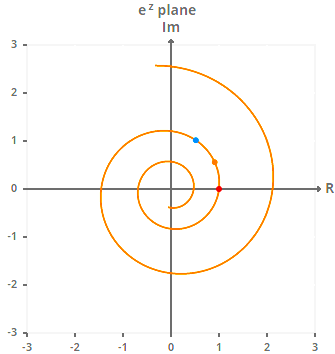
\includegraphics[width=0.25\textwidth]{./documents/l3/exp1.png}
            \caption{$\blac\operatorname{Sign}(a)=\operatorname{Sign}(b)$}
        }

        \ffigbox{
            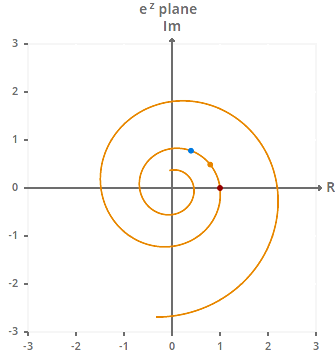
\includegraphics[width=0.25\textwidth]{./documents/l3/exp2.png}
            \caption{$\blac\operatorname{Sign}(a)\neq\operatorname{Sign}(b)$}
        }

    \end{floatrow}
\end{figure}

\subsection{Complex Polynomials}

Some polynomials with real coefficients, like $z^2+9$, can not be factored completely into degree 1 real polynomials, but do factor into degree 1 polynomials with complex coefficients: $(z+3i)(z-3i)$

\begin{tasks}(2)
    \task[] \hspace{-9mm}\uline{Real Polynomial:}\hspace{2mm} Polynomial with real coefficients
    \task[] \hspace{-12mm}\uline{Complex Polynomial:}\hspace{2mm} Polynomial with complex coefficients
\end{tasks}
\vspace{-10pt}

Every complex polynomial factors into degree 1 complex polynomials. This implies the following:\vspace{-7pt}

\begin{dent}{Fundamental Theorem of Algebra.}
    Every degree $n$ complex polynomial $f(z)$ has exactly $n$ complex roots if counted with multiplicity.
\end{dent}
\vspace{-6pt}

This will be useful for constructing solutions to higher-order linear ODEs with constant coefficients, and or discussing eigenvalues\vspace{-7pt}

\begin{dent}{Example.}
    Find the complex roots of $z^5=-32$

    Whenever we want to find roots of such equations we write in the polar form $z=re^{i\theta},\ r>0$\\
    Then we have : $\lr{e^{i\theta}}^{5}=32e^{i\pi}\eqi r^5e^{i5\theta}=32e^{i\pi}$\\
    The modulus of the roots must satisfy $r^5=32$ and the argument must satisfy $5\theta=\pi+2k\pi,\ \forall k\in\mathbb{N}$

    Thus $r=2$ and $\theta=\frac{\pi+2k\pi}{5},\ \forall k\in\mathbb{N}$, in other words $z=2e^{i(\pi+2k\pi)/5}$\\
    These are numbers on a circle of radius 2; to get from one to the next, rotate by $2\pi/5$. Increasing $k$ five times brings the number back to its original position. So its enough to take $k=0,1,2,3,4$
    \linecenter{$\boxed{S=\Bigl\{2e^{i\frac{\pi}{5}},2e^{i\frac{3\pi}{5}},2e^{i\pi},2e^{i\frac{7\pi}{5}},2e^{i\frac{9\pi}{5}}\Bigr\}}$}
\end{dent}

\begin{figure}[ht]
    \centering
    \begin{tikzpicture}
        \draw[-Stealth] (0,-2) -- (0,2);
        \draw[-Stealth] (-2,0) -- (2,0);
        \node at (0.3,2) {$\blac Im$};
        \node at (2,-0.3) {$\blac Re$};

        \node at (0.85,0.15) {\tiny1};

        \draw[color=blue] (0,0) circle (1.5);
        \draw[] (0,0) circle (0.75);

        \draw[color=green] (0,0) -- (1.2135,0.88167);
        \draw[color=green] (0,0) -- (-0.4635,1.4266);
        \draw[color=green] (0,0) -- (-1.5,0);
        \draw[color=green] (0,0) -- (-0.4635,-1.4266);
        \draw[color=green] (0,0) -- (1.2135,-0.88167);

        \filldraw[fill=red, color=red](1.2135,0.88167) circle (1.5pt);
        \filldraw[fill=red, color=red](-0.4635,1.4266) circle (1.5pt);
        \filldraw[fill=red, color=red](-1.5,0) circle (1.5pt);
        \filldraw[fill=red, color=red](-0.4635,-1.4266) circle (1.5pt);
        \filldraw[fill=red, color=red](1.2135,-0.88167) circle (1.5pt);


    \end{tikzpicture}
\end{figure}

\newpage

\section{Homogeneous Second-Order Linear Ordinary Differential Equation}

\subsection{Introduction}

Recall the spring-mass system from Lesson I, using Newton's law, we found that there is a second-order linear homogeneous differential equation that describes the displacement $x$ of the mass: $m\ddot{x}+kx=0$\\
Let us now look at the solutions to this equation. For simplicity $m=k=1$ such that $\ddot{x}+x=0$

The general principle behind the problem is that any linear combination of cosine and sine is a solution to $\ddot{x}+x=0\ :\ x(t)=C_1\cos(t)+C_2\sin(t),\ (C_1,C_2)\in\mathbb{C}^2$
This is a consequence of the superposition principle for a linear homogeneous differential equation:
\begin{dent}{}
    The solution to a linear homogeneous order $n$ equation $\mathcal{P}_n(t)y^{(n)}+\mathcal{P}_{n-1}(t)y^{(n-1)}+...+\mathcal{P}_0(t)y=0$
    have the following properties:
    \begin{items}{-13pt}{0pt}
        \item The zero function $0$ is a solution
        \item Multiplying any one solution to a scalar gives another solution
        \item Adding any two solutions gives another solution
    \end{items}
\end{dent}

\linecenter{$\boxed{\text{All linear combination of homogeneous solutions are homogeneous solutions}}$}

This is why homogeneous linear ODE are so nice. Later on, we'll see that the list of properties above means that the collection of all homogeneous solutions form what is known as a \red{vector space}.

The collection of all solutions to any second-order linear homogeneous differential equations is:
\linecenter{$x(t)=C_1x_1(t)+C_2x_2(t)$ where $x_1(t)$ and $x_2(t)$ are solutions to the second-order differential equation}

This two-parameter family of solutions is also called the general solution to the second-order linear differential equation.

\begin{dent}{Important :}
    $x_1(t)$ and $x_2(t)$ must be \red{linearly independent}. This means $x_1$ and $x_2$ cannot be a constant multiple of the other. In particular, this means neither $x_1$ nor $x_2$ can be zero.\\
    In this case, we can say that $x_1$ and $x_2$ form a \red{basis} for the set of all homogeneous solutions.\\
    \linecenter{(the definition of linear independence is more complicated for more than two elements)}
\end{dent}
\begin{dent}{Note :}
    There are \red{two} parameters in the general solution to a second-order differential equation roughly because to solve a second-order differential equation, in one way or another, we will find that in general, the number of arbitrary constants in the general solution corresponds to the order of a linear differential equation
\end{dent}

Every second-order linear ODE has a 2-parameter family of solutions. To nail down a specific solution, we need to specify two places of data for the solution. It is a beautiful fact that this data can be provided always by two initial conditions at the same starting time, such as $y(0)$ and $\dot{y}(0)$. The starting time could also be done by some number $a$ other than $0$.

Once we have found a basis $x_1$ and $x_2$ for the solutions, the initial conditions are satisfied by choosing the values for the two parameters $C_1$ and $C_2$.

\newpage

\subsection{Spring Mass Dash-pot system}

\begin{wrapfigure}[6]{r}{0.7\textwidth}
    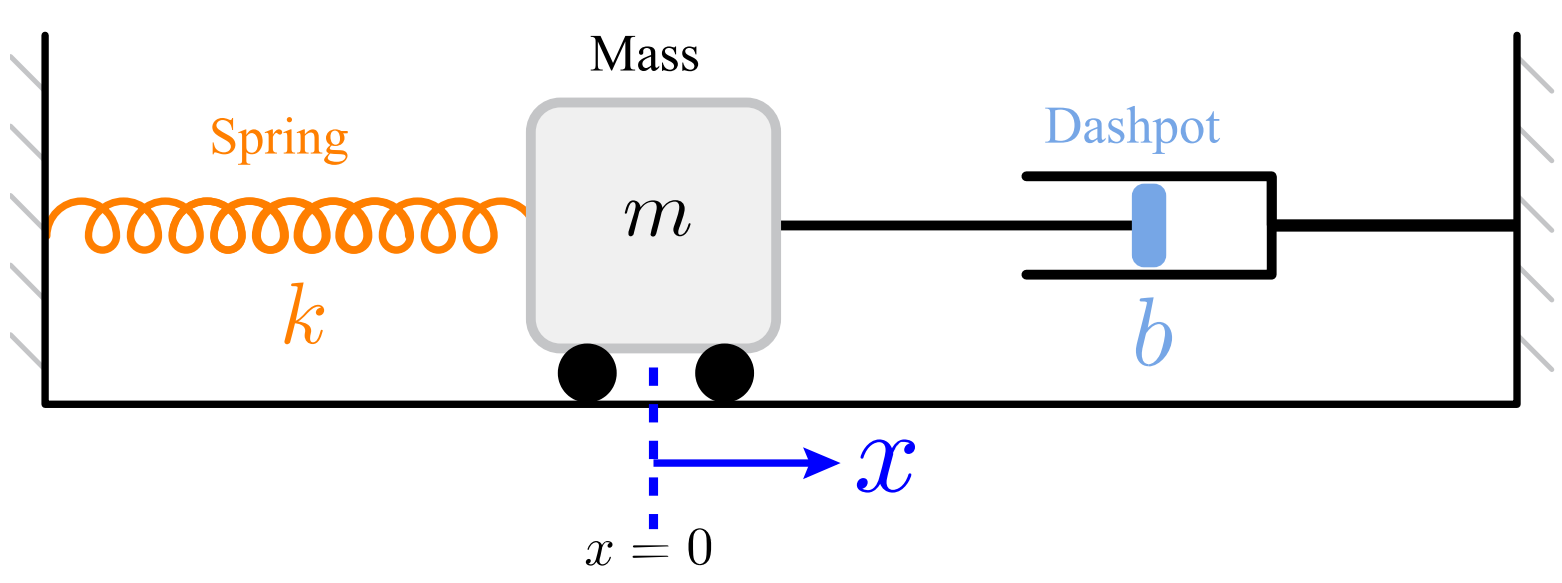
\includegraphics[width=0.65\textwidth]{./documents/l4/SPM-system.png}
\end{wrapfigure}

A mass sits on a cart that is attached to a wall by a small spring and a dash-pot, which is a damping device.

Find the differential equation for the position of the mass.
\begin{dent}{Defining variables :}
    \begin{items}{-10pt}{-10pt}
        \item $t$ time
        \item $x$ position of the mass, with $x=0$ being where the string exerts no force
        \item $m$ the mass
        \item $F_{spring}$ the force exerted by the spring on the mass
        \item $F_{dash-pot}$ the force exerted by the dash-pot on the mass
        \item $F$ total force exerted on the mass
    \end{items}

    $F_{spring}$ is a function of the position $x$, and has the opposite sign of $x$\\
    $F_{dash-pot}$ is a function of the velocity $x$, and has the opposite sign of $x$
\end{dent}

To simplify, we approximate these by linear functions : $F_{spring}=-kx,\ F_{dash-pot}=-b\dot{x}$ where $b$ is the damping constant

Using Newton's second law: $F=F_{spring}+F_{dash-pot}\eqi m\ddot{x}=-kx-b\dot{x}\eqi m\ddot{x}+b\dot{x}+kx=0$\vspace{-30pt}

\begin{dent}{}

    Input signal \hspace{8mm}: $0$ (no external forces on the mass)\\
    System\hspace{15.7mm} : spring, mass, dash-pot\\
    System response : $x(t)$
\end{dent}

In standard form : $\ddot{x}+\frac{b}{m}\dot{x}+\frac{k}{m}x=0$

When trying $x=e^{rt}$ as a solution we have $(mr^2+br+k)e^{rt}=0$\\
This holds equality if and only if $mr^2+br+k=0$, this is what we call the \red{characteristic equation}.\\
$\mathcal{P}(r)=mr^2+br+k$ is the \red{characteristic polynomial} of the given differential equation.

As usual for quadratic equations, there are three scenarios of the roots depending on the value of $\sqrt{b^2-4mk}$. Here we will discuss the general solutions to the differential equation in the case where the two roots are different, whether real or complex. Later we'll see when the roots are repeated.

\subsection{Two distinct real roots}

Consider the equation $\ddot{y}+5\dot{y}+6y=0$, the function $y=e^{rt}$ is a solution when $r$ is a root of the characteristic polynomial where $\mathcal{P}(r)=r^2+5r+6=(r+2)(r+3)$, the two functions $e^{-2t}$ and $e^{-3t}$ are solutions. Therefore, the general solution to the differential equation is $C_1e^{-2t}+C_2e^{-3t}$

For $y(0)=0 \implies C_1+C_2=0$ and for $\dot{y}(0)=0\implies-2C_1-3C_2=0$.\\
Solving this system we then find $C_1=1$ and $C_2=-1$

So the solution to the equation satisfying initial conditions is $y(t)=e^{-2t}-e^{-3t}$

\newpage

\subsection{Two distinct complex roots}

Suppose that the equation $\ddot{y}+A\dot{y}+By=0$ where $A$ and $B$ are real, has characteristic roots $a\pm ib$.

Since the characteristic roots are $a\pm ib$, the two complex exponents $e^{(a+ib)t}$ and $e^{(a-ib)t}$ form the basis of the collection of all solutions. Now, because all the coefficients in the differential equation are real, we then have:
\linecenter{$\Re\lr{e^{(a+ib)t}}=e^{at}\Re\lr{e^{ibt}}=e^{at}\cos(bt)$}
\linecenter{$\Im\lr{e^{(a+ib)t}}=e^{at}\Im\lr{e^{ibt}}=e^{at}\sin(bt)$}

These are also solutions to the differential equation. These two solutions are real and linearly independent, giving the general solution\\
\linecenter{$\boxed{y(t)=C_1e^{at}\cos(bt)+C_2e^{at}\sin(bt)}$}

If $y(t)=u(t)+iv(t)$ is a solution to a second-order homogeneous linear differential equation with real coefficients. Then plugging $y$ into the equation, we have:
\begin{eq}{-10pt}{-25pt}
    \blu (u+iv)''+A(u+iv)'+B(u+iv)=0\\
    \blu \implies (\ddot{u}+A\dot{u}+Bu)+i(\ddot{v}+A\dot{v}+Bv)=0
\end{eq}

\linecenter{\hspace{3mm}$\Red\overline{\quad\quad \textit{real}\ \ \ \quad} \qquad  \overline{\ \ \textit{imaginary}\ }$}

Since $A$ and $B$ are real, the real and imaginary parts of the differential equation are respectively enclosed in the two parts above, and therefore both $u$ and $v$ are solutions to the original differential equation. \\
Note that it is crucial in this last step that all coefficients of the differential equation are real.

\subsection{Spring Mass Solution}

Using what we've seen let's proceed to solve our original problem $\ddot{y}+y=0$ without the dash-pot.\\
The characteristic equation becomes $r^2+1=0$ with roots $i$ and $-i$. Thus the exponential solution $e^{it}$ and $e^{-it}$ form a basis for the collection of all solutions.

Since the coefficients are real we then have solutions $\Re\lr{e^{it}}=\cos(t)$ and $\Im\lr{e^{it}}=\sin(t)$, and since both are linearly independent $\cos(t)$ and $\sin(t)$ form another basis for the collection of all solutions.

The general real solution is all real linear combinations of these two basic functions:
\linecenter{$\boxed{y(t)=C_1\cos(t)+C_2\sin(t)}$}

This is the same solution we hinted at the beginning of this lesson

\begin{dent}{Note :}
    The same solution can be obtained using complex solutions.\\
    Let $z=e^{it}$ then $\overline{z}=e^{-it}$. By combination, we can then obtain the real and imaginary parts:
    \linecenter{$\ds{\Re(z)=\frac{z+\overline{z}}{2}}$ and $\ds{\Im(z)=\frac{z-\overline{z}}{2i}}$}

    Becoming $\ds{\Re(z)=\frac{e^{it}+e^{-it}}{2}=\cos(t)\ ;\ \Im(z)=\frac{e^{it}-e^{-it}}{2i}=\sin(t)}$
\end{dent}

Taking the linear combination of both solutions we then have the real solutions $C_1\cos(t)+C_2\sin(t)$.\\
Provided $C_1$ and $C_2$ are complex values.

The basis that should be used depends:
\begin{items}{-15pt}{-10pt}
    \item The basis $e^{it}$, $e^{-it}$ is easier to calculate with, but we need to be careful with which linear combinations of the expression of these functions are real-valued.
    \item The basis $\cos(t)$, $\sin(t)$ is useful for integrating solutions in a physical system.
\end{items}

\newpage

\subsection{Coefficients for the real solution}

Once we have the solution $C_1e^{(a+ib)t}+C_2e^{(a-ib)t}$ we can find a solution $u+iv$ such that $v=0$. Another way to look for real solutions is finding a value for which $z=\overline{z}$:\vspace{-25pt}
\begin{dent}{}

    We then have : $\overline{C_1}e^{(a+ib)t}+\overline{C_2}e^{(a-ib)t}$

    Therefore $\overline{C_1}=C_2$ or $C_1=\overline{C_2}$ which gives $(c+id)e^{(a+ib)t}+(c-id)e^{(a-ib)t}$
\end{dent}

Converting back to $\sin/\cos$ we can use the following method:
\begin{eq}{-10pt}{-20pt}
    \blu (c+id)e^{(a+ib)t}+(c-id)e^{(a-ib)t} &\blu= e^{at}\Big(c\big(e^{ibt}+e^{-ibt}\big)+id\big(e^{ibt}-e^{-ibt}\big)\Big) \\
    &\blu= e^{at}\Big(2c\cos(bt)+id\big(2i\sin(bt)\big)\Big) \\
    &\blu= e^{at}\Big(2c\cos(bt)-2d\sin(bt)\Big)
\end{eq}

Taking once more the form $C_1\cos(bt)+C_2\sin(bt)$
\begin{dent}{Example 1 :}
    Lets consider $\ddot{x}+5\dot{x}+4x=0$.\\
    The characteristic equation is $R^2+r+1=0$ with roots $r=-1$ and $r=-4$.\\
    The basis for the solution is $e^{-t}$ and $e^{-4t}$ therefore the general solution is the form of these two solutions which in a general form can be written as a linear combination:\\
    \linecenter{$\boxed{x(t)=C_1e^{-t}+C_2e^{-4t}}$}
\end{dent}

\begin{dent}{Example 2 :}
    Lets consider $\ddot{x}+\dot{x}+x=0$.\\
    The characteristic equation is $r^2+r+1=0$ with roots $r=-\frac{1}{2}+i\frac{\sqrt{3}}{2}$ and $r=-\frac{1}{2}-i\frac{\sqrt{3}}{2}$.\\
    The basis for the complex exponential solution are $z=e^{\frac{(-1+i\sqrt{3})}{2}t}$ and $z=e^{\frac{(-1-i\sqrt{3})}{2}t}$ therefore the basis of all real solutions becomes:
    \linecenter{$x_1=e^{-t/2}\cos(\frac{\sqrt{3}}{2}t)\ ;\ x_2=e^{-t/2}\sin(\frac{\sqrt{3}}{2}t)$}

    This brings us to our general solution:
    \linecenter{$\boxed{x(t)=e^{-t/2}\big(C_1\cos(\frac{\sqrt{3}}{2}t)+C_2\sin(\frac{\sqrt{3}}{2}t)\big)}$}
\end{dent}

\begin{dent}{Example 3 :}
    Lets consider $\ddot{x}+4\dot{x}+5x=0$.\\
    The characteristic equation is $R^2+4r+5=0$ with roots $r=-2+t$ and $r=-2-i$.\\
    The basis for the solution are then then$z=e^{(-2+i)t}$ and $z=e^{(-2-i)t}$.The general solution is a linear combination of these two solutions.\\
    But because the differential equation has real coefficients, we were expecting real-valued solutions. Instead, we can take the basis formed by the real and imaginary part of $z$:
    \linecenter{$z=e^{(-2+i)t}=e^{-2t}\cos(t)+i\sin(t)$}

    Now we can have a basis of two real-valued functions and can use the superposition principle to find the general real-valued solution:
    \linecenter{$x(t)=C_1e^{-2t}\cos(t)+C_2e^{-2}\sin(t)$}

    If we take the basis of two real valued function $\overline{z}$, then we would have:
    \linecenter{$\overline{z}=e^{-2t}\cos(t)-ie^{-2t}\sin(t)$}

    Bringing us back to : $x(t)=C_1e^{-2t}\cos(t)+C_2e^{-2t}\sin(t)$\\
    Solutions from $z$ or $\overline{z}$ work the same
\end{dent}

\chapter{Damped Functions}

\section{Lesson V: Sinusoidal Functions}

\subsection{Introduction}

Recall that the position of the mass-spring-dashpot system without external force can be modeled by the second-order linear homogeneous ODE: $m\ddot{x}+b\dot{x}+kx=0$

Let the damping constant be small enough so that $b^2<4mk$ and the characteristic polynomial has 2 distinct complex roots. The real basis that gives the real solution is then:
\linecenter{$x(t)=e^{\frac{-b}{2m}t}\big(C_1\cos(\omega t)+C_2\sin(\omega t)\big)\ ,\ (C_1,C_2)\in\mathbb{R}$}

With $\omega=\sqrt{\frac{k}{m}-\frac{b^2}{4m^2}}$ called the damped frequency of the system.

Contrasting the solution to the general spring mass system $m\ddot{x}+kx=0$ we then have $x(t)=C_1\cos(\omega_n t)+C_2\sin(\omega_n t)$ where $\omega_n$ is called the natural frequency of the system.\\
Even if $b>0$ we will keep calling $\omega_n$ the natural frequency.

\subsection{From rectangular to polar form}

There are two ways of expressing any sinusoidal function, in \red{rectangular form}, and in \red{polar form}, related as follows:

\begin{wrapfigure}[10]{l}{0pt}
    \begin{tikzpicture}[scale=1.35]
        \draw[] (-2,0) -- (2,0);
        \draw[] (0,-0.5) -- (0,2);

        \draw[color=red] (0,0) -- (1.5,1.75);
        \filldraw[fill=black] (1.5,1.75) circle (2pt);

        \draw[dashed] (0,1.75) -- (1.5,1.75);
        \draw[dashed] (1.5,0) -- (1.5,1.75);

        \draw[red, -latex] (0.5,0) arc (0:49.4:0.5);

        \node at (-0.3,1.75) {b};
        \node at (1.5,-0.3) {a};
        \node at (0.65, 0.3) {$\red{\phi}$};
        \node at (2,1.9) {(a,b)};
        \node[rotate=49.4] at (0.65,1) {$\red{A}$};

        \draw[] (-2,-2) -- (2,-2);
        \draw[] (0,-1.5) -- (0,-4);

        \draw[color=red] (0,-2) -- (-1,-3.732);
        \filldraw[fill=black] (-1,-3.732) circle (2pt);

        \draw[dashed] (0,-3.732) -- (-1,-3.732);
        \draw[dashed] (-1,-2) -- (-1,-3.732);

        \draw[red, -latex] (0.5,-2) arc (0:-120:0.5);

        \node at (0.3,-3.732) {$\blac-\sqrt{3}$};
        \node at (-1,-1.7) {$\blac-1$};
        \node at (0.65, -2.3) {$\red{\frac{2\pi}{3}}$};
        \node at (-1.4,-4) {($\blac-1,-\sqrt{3}$)};
        \node[rotate=60] at (-0.65,-2.7) {$\red{2}$};


    \end{tikzpicture}
\end{wrapfigure}

\begin{eq}{-10pt}{-10pt}
    \blu a\cos(\theta)+b\sin(\theta)&\blu=\red{A}\cos(\theta-\red{\phi})\\
    &\blu=\red{A}\cos(\red{\phi})\cos(\theta)+\red{A}\sin(\red{\phi})\sin(\theta)
\end{eq}

In practice, the argument of the cosine and sine terms is often a function rather than a constant. Usually we have: $\theta=\omega t$ for $\omega>0$.


\begin{dent}{Example :}
    Converting $-\cos(5t)-\sqrt{3}\sin(5t)$

    Given $a=-1$, $b=-\sqrt{3}$, $\theta(t)=\omega t$ where $\omega =5$\\
    We then have $A=\sqrt{(-1)^2+(-\sqrt{3})^2}=2$ and $\phi=-\frac{2\pi}{3}$

    Therefore $-\cos(5t)-\sqrt{3}\sin(5t)=2\cos(5t+\frac{2\pi}{3})$

\end{dent}

\newgeometry{width=18.625cm, bottom=2cm, top=2cm}

\subsection{Proof of the trigonometric identities}

There are three different ways to write a sinusoidal function of angular frequency $\omega$ :
\begin{items}{-10pt}{-10pt}
    \item Amplitude-phase form : $A\cos(\omega t -\phi)$, where $A$ and $\phi$ are real numbers with $A\geq 0$.
    \item Complex form : $\Re\big(Ce^{i\omega t}\big)$ where $C$ is a complex number.
    \item Linear combination : $a\cos(\omega t)+b\sin(\omega t)$ where $a$ and $b$ are real numbers
\end{items}

Different forms are useful in different contexts, so we'll need to know how to convert between them.
\begin{dent}{}
    If $\overline{C}=Ae^{i\phi}=a+ib$ where $C\in\mathbb{C}$, $A\geq0$, $(a,b)\in\mathbb{R}$, then $\Re\big(Ce^{i\omega t}\big)=A\cos(\omega t-\phi)=a\cos(\omega t)+b\sin(\omega t)$
    \linecenter{($\overline{C}$ is the complex conjugate form of $C$)}
\end{dent}

\begin{dent}{Proofs}
    \begin{tasks}(2)
        \task[1.]
        \begin{lfeq}{-27pt}{-27pt}
            \blu\Re\big(Ce^{i\omega t}\big)&\blu=\Re\big(Ae^{-i\phi}e^{i\omega t}\big)&\\
            &\blu=\Re\big(Ae^{i(\omega t-\phi)}\big)&\\
            &\blu=A\cos(\omega t-\phi)
        \end{lfeq}

        \task[2.]
        \begin{lfeq}{-27pt}{-27pt}
            \blu\Re\big(Ce^{i\omega t}\big)&\blu=\Re\lr{(a-ib)\big(\cos(\omega t)+i\sin(\omega t)\big)}&\\
            &\blu=\Re\big(a\cos(\omega t)+b\sin(\omega t) +i(...)\big)&\\
            &\blu=\cos(\omega t)+b\sin(\omega t)
        \end{lfeq}
    \end{tasks}
    \begin{tasks}
        \task[3.]Using $\cos(x-y)=\cos(x)\cos(y)+\sin(x)\sin(y)$ we have
        \begin{eq}{-10pt}{-27pt}
            \blu A\cos(\omega t-\phi)&\blu=A\cos(\omega t)\cos(\phi)+A\sin(\omega t)\sin(\phi)\\
            &\blu=a\cos(\omega t)+b\sin(\omega t)
        \end{eq}
    \end{tasks}
    \begin{tasks}
        \task[4.]
        \begin{lfeq}{-24pt}{-27pt}
            \blu a\cos(\omega t)+b\sin(\omega t)&\blu=(a,b)\cdot\big(\cos(\omega t),\sin(\omega t)\big)&\\
            &\blu=|(a,b)||\big(\cos(\omega t),\sin(\omega t)\big)|\cos\big((\overrightarrow{a,b}),(\overrightarrow{\cos(\omega t),\sin(\omega t)})\big)&\\
            &\blu=A\cos(\omega t -\phi)
        \end{lfeq}
    \end{tasks}
\end{dent}

In polar form, it is easy to see that the graph of the sinusoidal function $f(t)=A\cos(\omega t -\phi)$ is a rescaled and shifted version of the cosine graph.

The graph of $f(t)$ can be described geometrically by:
\begin{items}{-10pt}{-10pt}
    \item $\red{A}$, its $\red{amplitude}$, how high the graph rises above the $t$-axis at its maximum.
    \item $\red{P}$, its $\red{period}$, the time for one complete oscillation, or width between successive maxima
    \item $\red{t_0}$, its time lag, a $t$-value ate which a maximum is attained $t_0=\frac{\phi}{\omega}$ since $\omega t-\phi=0$
\end{items}

\subsection{Sketching the solution to an under-damped spring-mass-dashpot system}

In the previous chapter, we've seen how to find the general solution to the spring-mass dash-pot system with $m=1$, $b=4$, $k=5$ and $y_0=1$, $\dot{y}_0=0$ where the solution is $y=e^{-2t}\big(\cos(t)+2\sin(t)\big)$

Using the trigonometric identities as seen previously the following equation becomes: $y=\sqrt{5}e^{-2t}\cos(t-\phi)$
\begin{figure}[ht]
    \centering
    \begin{tikzpicture}[scale=0.7]
        \draw[-Stealth] (-0.5,0) -- (10,0);
        \draw[-Stealth] (0,-2.5) -- (0,2.5);

        \draw[color=blue, domain=0:10, smooth, samples=100] plot ({\x},{sqrt(5)*exp(-2*\x/4)*cos(2.5*\x r -1.107 r)});

        \draw[dashed , domain=0:10, smooth, samples=100] plot ({\x},{sqrt(5)*exp(-2*\x/4)});
        \draw[dashed , domain=0:10, smooth, samples=100] plot ({\x},{-sqrt(5)*exp(-2*\x/4)});

        \draw[] (8,1) -- (9,1) -- (9,2.5) -- (8,1);
        \draw[] (8.5,1) arc (0:57:0.5);
        \node at (8.5,0.5) {$\blac1$};
        \node at (9.5,1.75) {$\blac2$};
        \node[rotate=57] at (8.1,1.95) {$\blac\sqrt{5}$};
        \node at (8.7,1.5) {$\blac\phi$};
        \node at (11.5,1.75) {$\blac\phi\approx64^{\circ}$};

        \filldraw[fill=black] (0,1) circle (2pt);

        \draw[-latex] (2,1.6) arc (90:150:0.7);
        \draw[] (0.4,-0.1) -- (0.4,0.1);

        \node at (-0.3,1) {$\blac1$};
        \node at (3,1.6) {$\blac\sqrt{5}e^{-2t}$};
        \node at (0.5 ,-0.5) {$\blac\frac{\pi}{2}$};

    \end{tikzpicture}
\end{figure}

\newpage

The main difference between solutions to a damped and an undamped system (where $b$ is small enough so there are two complex roots) is that real solutions to the damped system have an additional overall exponential factor.

The general solution to $m\ddot{y}+b\dot{y}+ky=0$ (where $b^2<4mk$) is:
\begin{eq}{-10pt}{-27pt}
    \blu y&\blu=e^{(-\frac{b}{2m})t}\big(C_1\cos(\omega_d t)+C_2\sin(\omega_d t)\big)\\
    &\blu=Ae^{(-\frac{-b}{2m})t}\cos(\omega_d t-\phi)
\end{eq}

This is the system's response for an unforced spring mass dash-pot system and is what we call the \red{damped sinusoid}.\\
Furthermore, $x(t)$ crosses the equilibrium whenever the pure sinusoid $\cos(\omega t-\phi)$ does. Thus the period $P$ and time lag $t_0$ still make sense and have the same formulas as for the pure sinusoid: $P=\frac{2\pi}{\omega}$ and $t_0=\frac{\phi}{\omega}$

Because $x(t)$ is not truly periodic (its amplitude decreases), we call $P$ the \red{pseudo-period}.

\begin{dent}{Example.}
    Consider two sinusoid sound waves of angular frequencies $\omega+\epsilon$ and $\omega-\epsilon$, say $\epsilon<<\omega$\\
    What happens when they are superposed?
    \begin{eq}{-10pt}{-27pt}
        \blu \cos((\omega+\epsilon)t)+\cos((\omega-\epsilon)t)&\blu=\Re\big(e^{i(\omega+\epsilon)t}\big)+\Re\big(e^{i(\omega-\epsilon)t}\big)\\
        &\blu=\Re\big(e^{i\omega t}(e^{i\epsilon t}+e^{-i\epsilon t})\big)\\
        &\blu=2\cos(\omega t)\cos(\epsilon t)
    \end{eq}

    The function $\cos(\omega t)$ oscillates rapidly between $\pm 1$. Multiplying it by the now slowly varying function $2\cos(\epsilon t)$ produces a rapid oscillation between $\pm 2\cos(\epsilon t)$, so one hears a sound wave of angular frequency $\omega$ whose amplitude is the slowly varying $|2\cos(\epsilon t)|$
\end{dent}

\begin{figure}[ht]
    \centering
    \begin{tikzpicture}[scale=0.8]
        \draw[-Stealth] (0,0) -- (10.2,0);
        \node at (10.2,-0.4) {$\blac t$};

        \draw[smooth, color=blue, samples=500, domain=0:10] plot ({\x},{2*cos(\x r)*cos(16*\x r)});
    \end{tikzpicture}
\end{figure}

You hear beats when tuning the strings of an instrument. The oscillating sound is exactly these beats. The higher the frequency of the beat the more out of tune. As instruments or strings become closer and closer in tune, the frequency of the beats diminishes until you can't hear them at all.

Changing the phase of one signal with respect to the other doesn't change the frequency of the beat. This is important.

\newpage

\section{Lesson VI: Damped Harmonic Oscillations}

\subsection{Damping}

If there is no damping, the differential equation that models the position of the mass is $m\ddot{x}+kx=0$ owning real-valued solution $a\cos(\omega_n t)+b\sin(\omega_n t)$ or $A\cos(\omega_n t-\phi)$\\
In other words, this system, or any other system governed by the same equation is called a simple harmonic oscillator. The angular frequency $\omega_n$ is also called the natural frequency (or resonant frequency) of the oscillator.

If damping is present, the differential equation that models the position of the mass is $m\ddot{x}+b\dot{x}+kx=0$\\
This brings us to the characteristic polynomial $\mathcal{P}(r)=mr^2+br+k$ with roots being:
\linecenter{$r_0=-\frac{b}{2m}\pm\sqrt{\lr{\frac{b}{2m}}^2-\omega_{n}^2}$}

Depending on the sign of $\lr{\frac{b}{2m}}^2-\omega_{n}^2$ we can separate 3 different cases. The behavior of the solution in these 3 cases is qualitatively different.

\begin{dent}{Case 1: $b^2<4mk$ underdamped} There are 2 complex roots, and we will give names to the real and imaginary parts. Since the real part is always negative, we call it $-p$, with $p=\frac{b}{2m}$. The imaginary part is either the positive or negative of the \red{damped frequency}, $\omega_d$ given by $\omega_d=\sqrt{\omega_{n}^2-p^2}$

    The general solution then found will be $e^{pt}\lr{a\cos(\omega_d t)+b\sin(\omega_d t)}$ or $Ae^{-pt}\cos(\omega_d -\phi)$.\\
    This is a sinusoid multiplied by a decaying exponential. Each non-zero solution tends to 0, but changes sign infinitely many times along the way. The system is called \red{underdamped} because there is not enough damping to eliminate the oscillations.\\
    The damping not only causes the solution to decay exponentially but also changes the frequency of the sinusoid. The new angular frequency $\omega_d$ is what we call the \red{damped frequency}.\\
    It is less than the natural frequency as evident from the formula $\omega_d=\sqrt{\omega_{n}^2-p^2}$.\\
    The damped solutions are not periodic, they don't repeat exactly because of the decay. Therefore $\frac{2\pi}{\omega_d}$ is called the pseudo period.

\end{dent}
\begin{figure}[ht]
    \centering
    \begin{tikzpicture}[scale=1]
        \draw[-Stealth] (-0.5,0) -- (10,0);
        \draw[-Stealth] (0,-2.5) -- (0,2.5);

        \draw[color=blue, domain=0:9.8, smooth, samples=100] plot ({\x},{sqrt(5)*exp(-2*\x/4)*sin(2.5*\x r)});

        \draw[dashed , domain=0:9.8, smooth, samples=100] plot ({\x},{sqrt(5)*exp(-2*\x/4)});
        \draw[dashed , domain=0:9.8, smooth, samples=100] plot ({\x},{-sqrt(5)*exp(-2*\x/4)});

        \draw[-latex] (2,1.6) arc (90:150:0.7);
        \draw[latex-latex] (0.2,0.15) -- (2.3,0.15);
        \draw[-latex] (3.5,1.2) arc (90:135:3);

        \node at (4,1.2) {$\blac\frac{2\pi}{\omega_d}$};
        \node at (2.7,1.8) {$\blac e^{-pt}$};
    \end{tikzpicture}
\end{figure}

\newpage

\begin{dent}{Case 2 : $b^2>4mk$ overdamped}
    In this case, the roots $\frac{-b\pm\sqrt{b^2-4mk}}{2m}$ are real and distinct. Both roots are negative, since $\sqrt{b^2-4mk}<b$. We'll call them $-s_1$ and $-s_2$.\\
    The general solution found will have the form $ae^{-s_1t}+be^{-s_2t}$ where $a$, $b$ are real constants.\\
    As in all the other damped cases, all solutions 0 tend to as we go to infinity. The term corresponding to the \red{less negative} root eventually controls the rate of return to equilibrium. The system is called \red{overdamped}; there is so much damping that it is
    slowing the return to equilibrium.\\
    Because of the important damping, the function can cross the equilibrium at most once.
    \begin{dent}{Proof :} Let there be a time $t_0$ for which the system is at equilibrium.\\
        This would mean that $x(t_0)=ae^{-s_1t_0}+be^{-s_2t_0}=0$.

        Solving for $t_0$ we would then obtain $\ds{t_0=\frac{\ln\lr{-\frac{a}{b}}}{s_1-s_2}}$

        With this, we can see that if $-\frac{a}{b}$ is negative, there is no point for $t_0>0$ where the function will cross the equilibrium. If it is positive then there will only exist 1 solution for which the function crosses the equilibrium.
    \end{dent}

    \begin{figure}[ht]
        \centering
        \begin{tikzpicture}
            \draw[-Stealth] (-0.5,0) -- (10,0);
            \draw[-Stealth] (0,-2.5) -- (0,2.5);

            \draw[color=blue, domain=0:9.8, smooth, samples=100] plot ({\x},{exp(-1.5*\x)+exp(-0.5*\x)});
            \draw[color=orange, domain=0:9.8, smooth, samples=100] plot ({\x},{5*exp(-0.5*\x)-4*exp(-1.5*\x)});
            \draw[color=red, domain=0:9.8, smooth, samples=100] plot ({\x},{5*exp(-1.5*\x)-4*exp(-0.5*\x)});
            \draw[color=violet, domain=0:9.8, smooth, samples=100] plot ({\x},{-5*exp(-0.5*\x)+4*exp(-1.5*\x)});

            \node at (8,2.5) {$\color{blue}0<a<b$ \textcolor{blue}{and} $\color{blue}s_1>s_2$};
            \node at (8,2) {$\color{orange}b<0<a$ \textcolor{orange}{with} $\color{orange}|a|>|b|$ \textcolor{orange}{and} $\color{orange}s_1>s_2$};
            \node at (8,1.5) {$\color{red}b<0<a$ \textcolor{red}{with} $\color{red}|a|>|b|$ \textcolor{red}{and} $\color{red}s_1<s_2$};
            \node at (8,1) {$\color{violet}b<0<a$ \textcolor{violet}{with} $\color{violet}|a|<|b|$ \textcolor{violet}{and} $\color{violet}s_1>s_2$};

        \end{tikzpicture}
    \end{figure}

    This criterion gives one way to distinguish between underdamped and overdamped oscillators. In the underdamped case, the oscillations continue indefinitely. In the overdamped case, there are no oscillations at all.

\end{dent}

\begin{dent}{Case 3 : $b^2=4mk$ critically damped}
    The critically damped case happens at the border between the underdamped case and the overdamped case.\\
    There is a repeated real root, which we denote by $-p$ with $p=\frac{b}{2m}$ as before. The repeated root gives only one exponential solution $e^{-\frac{bt}{2m}}$.\\
    For a homogeneous second-order linear differential equation with repeated characteristic roots $r$, the basis of the solutions is $e^{rt}$ and $te^{rt}$

    Therefore the general solution takes the form $C_1e^{rt}+C_2te^{rt}$ or also put:
    \linecenter{$\boxed{e^{-pt}(a+bt)}$ where $a$ and $b$ are real constants }

    As we tend to infinity the exponential factor tends to 0, thus all solutions eventually decay. \\
    This case is when there is just enough damping to eliminate the oscillation. The system is called \red{critically damped}.

    \newpage

    \begin{dent}{Proof :}
        Consider $\ddot{y}+2a\dot{y}+a^2y=0$.

        Using the characteristic equation we can quickly find that the solution of this equation is $y_1=e^{-at}$. This causes an issue since we're expecting to have 2 different solutions in a second-order differential equation.

        Therefore we introduce the function $u(t)$ as a variation of parameter such that $y=y_1u(t)$, this in turn gives:
        \begin{eq}{-10pt}{-40pt}
            \blu y&\blu=e^{-at}u\\
            \blu \dot{y}&\blu=-ae^{-at}u+e^{-at}\dot{u}\\
            \blu \ddot{y}&\blu=a^2e^{-at}u-2ae^{-at}\dot{u}+e^{-at}\ddot{u}\\
        \end{eq}

        As we multiply each term by its respectful coefficient we obtain the following differential equation:\\
        \linecenter{$e^{-at}\ddot{u}=0$}

        The solution simply being $u(t)=C_1t+C_2$.\\
        From this family of solutions, $u(t)=t$ is simple enough to give a solution that is different from our previous one. Therefore $y=te^{-at}$

    \end{dent}

\end{dent}

\subsection{Sum-up}

As a general rule, we can use the following table for reference:\vspace{-10pt}\\
\begin{figure}[ht]
    \renewcommand{\arraystretch}{1.5}
    {\setlength{\tabcolsep}{2em}
        \begin{tabular}{c c l}
            \textbf{Case} & \textbf{Roots}                        & \textbf{Situation}                    \\
            $b=0$         & two complex roots $\pm i\omega_n$     & undamped (simple harmonic oscillator) \\
            $b^2<4mk$     & two complex roots $-p\pm i\omega_d$   & underdamped (damped oscillator)       \\
            $b^2=4mk$     & repeated real root $-p_1$,$-p$        & critically damped                     \\
            $b^2>4mk$     & distinct real roots $-s_1$ and $-s_2$ & overdamped                            \\
        \end{tabular}}
\end{figure}

\begin{figure}[ht]
    \begin{tikzpicture}
        \draw[-Stealth] (-0.5,0) -- (10,0);
        \draw[-Stealth] (0,-4) -- (0,4);

        \draw[color=black, domain=0:9.8, smooth, samples=100] plot ({\x},{3*(cos(\x r)+1/sqrt(3)*sin(\x r))});
        \draw[color=blue, domain=0:9.8, smooth, samples=100] plot ({\x},{3*(exp(-0.5*\x)*(cos(\x*sqrt(3)/2 r)+1/sqrt(3)*sin(\x*sqrt(3)/2 r)))});
        \draw[color=orange, domain=0:9.8, smooth, samples=100] plot ({\x},{3*(exp(-\x)*(1+\x))});
        \draw[color=red, domain=0:9.8, smooth, samples=100] plot ({\x},{3*((1/2+3/(2*sqrt(5)))*exp((-3+sqrt(5))/2*\x)+(1/2-3/(2*sqrt(5)))*exp((-3-sqrt(5))/2*\x))});

        \node at (7,-1) {\textcolor{black}{undamped}};
        \node at (7,-1.5) {\textcolor{blue}{underdamped}};
        \node at (7,-2) {\textcolor{orange}{critically damped}};
        \node at (7,-2.5) {\textcolor{red}{overdamped}};

    \end{tikzpicture}
\end{figure}

\newpage

\subsection{Stability of a boat}

A boat rocking from side to side is subjected to one of two cases, either \red{stable} or \red{unstable} motion. The stability of the boat will determine if it either capsizes or settles down to equilibrium. This, as we'll see, is determined by specific parameters involving the design of the boat.

To properly model this rocking effect we'll be using Newton's second law for the rotational motion: $\boxed{\tau=I\ddot{\theta}}$

As it rocks we observe that the induced torque varies along $\theta$

\begin{figure}[ht]
    \begin{floatrow}
        \ffigbox{
            % Boat
            \begin{tikzpicture}
                \draw[rotate=-20] (2,1.25) -- (2,-0.75);
                \draw[rotate=-20] (-2,1.25) -- (-2,-0.75);
                \draw[rotate=-20, decorate, decoration={brace,amplitude=15pt}, xshift=0cm, yshift=0pt] (2,-0.75) -- (-2,-0.75);
                \draw[rotate=-20, dashed, color=cyan] (-2.5,0) -- (2.5,0);
                \draw[color=cyan] (-2.5,0) -- (2.5,0);
                \draw[-latex] (1.25,0) arc (0:-20:1.25);
                \node at (1.45,-0.25) {$\blac\theta$};

            \end{tikzpicture}}

        \ffigbox{
            % Plot
            \begin{tikzpicture}
                \draw[-Stealth] (0,-1.5) -- (0,1.5);
                \draw[-Stealth] (-2,0) -- (2,0);

                \draw[color=blue, domain=-1:1, smooth, samples=100, rotate=90] plot ({\x},{1.5*tanh(2*\x)});
                \draw[color=black, domain=-1.25:1.25, smooth, samples=100, dashed, rotate=115] plot ({\x},{\x});

                \node at (0.5,1.5) {$\blac\tau(\theta)$};
                \node at (2,0.3) {$\blac\theta$};
                \node at (-2.5,0.75) {$\blac\tau\approx-k\theta$};
            \end{tikzpicture}}

    \end{floatrow}
\end{figure}
As we can see, we can approximate the torque using measured values as $\theta$ changes. This allows us to describe the system with the following differential equation: $I\ddot{\theta}+k\theta=0$.\\
This is a simple harmonic oscillator with period $\ds{p=\frac{2\pi}{\sqrt{\frac{k}{I}}}}$\\
The system is in a \red{stable} equilibrium, the boat isn't at risk of capsizing.

If however $k$ becomes negative then the differential equation will resemble $I\ddot{\theta}-|k|\dot{\theta}$.\\
In this case, $\theta$ will grow exponentially. Therefore the system is in an \red{unstable} equilibrium.

\subsection{Effects of boat shape}

For the previous equation $I\ddot{\theta}+k\theta=0$ to be useful to us we need to figure out how the constant $k$ varies according to the geometric parameters of the boat.\\
In this system we need to account for both the gravitational forces $\overrightarrow{F_G}$ and the buoyancy $\overrightarrow{F_B}$ applied to the system.

\begin{figure}[ht]
    \begin{floatrow}
        \ffigbox{
            \begin{tikzpicture}
                % boat
                \draw[] (-2.5,2) -- (-2.5,-1.5);
                \draw[] (2.5,2) -- (2.5,-1.5);
                \draw[color=cyan] (-3.5,0) -- (3.5,0);
                \draw[decorate, decoration={brace,amplitude=15pt}, xshift=0cm, yshift=0pt] (2.5,-1.5) -- (-2.5,-1.5);

                \fill[fill=cyan, opacity=0.075] (-2.3,-1.75) -- (-2.5,-1.65) -- (-2.5,0) -- (2.5,0) -- (2.5,-1.725);

                \draw[dashed,opacity=0.5] (0,1.5) -- (0,-2);

                \filldraw[color=red!100!white!50, fill=red!100!white!50] (0,1) circle (2pt);
                \draw[-Latex, color=red!100!white!50] (0,1) -- (0,0.15);

                \filldraw[color=blue!100!white!50, fill=blue!100!white!50] (0,-1) circle (2pt);
                \draw[-Latex, color=blue!100!white!50] (0,-1) -- (0,-0.15);

                \draw[Latex-Latex, color=yellow!40!orange] (-0.3,1) -- (-0.3,-1);
                \node at (-0.6,0.2) {$\color{yellow!40!orange}D$};

                \draw[Latex-Latex, color=yellow!40!orange] (-2.5,-2.3) -- (2.5,-2.3);
                \node at (0,-2.6) {$\color{yellow!40!orange}b$};

                \node at (0.3,1.2) {$\color{red!100!white!50}C_G$};
                \node at (0.3,0.5) {$\color{red!100!white!50}\overrightarrow{F_G}$};
                \node at (0.3,-1.2) {$\color{blue!100!white!50}C_B$};
                \node at (0.3,-0.5) {$\color{blue!100!white!50}\overrightarrow{F_B}$};
                \node at (-1.5,-0.75) {\Large$\color{cyan!70}A$};

                \node at (0,1.75) {\Large$\color{red!90}\tau=0$};

            \end{tikzpicture}}

        \ffigbox{
            \begin{tikzpicture}
                % boat
                \draw[rotate=-20,anchor=center] (-2.5,2) -- (-2.5,-1.5);
                \draw[rotate=-20] (2.5,2) -- (2.5,-1.5);
                \draw[dashed, rotate=-20, color=cyan] (-3.5,0) -- (3.5,0);
                \draw[color=cyan] (-3.5,0) -- (3.5,0);
                \draw[rotate=-20, decorate, decoration={brace,amplitude=15pt}, xshift=0cm, yshift=0pt] (2.5,-1.5) -- (-2.5,-1.5);

                \fill[fill=cyan, opacity=0.075] (-2.9,-0.8) -- (-2.65,0) -- (2.65,0) -- (1.7,-2.5) -- (-2.9,-0.8);

                \draw[rotate=-20, dashed,opacity=0.5] (0,1.5) -- (0,-2);

                \draw[dashed, opacity=0.5] (0.34,1.5) -- (0.34,-1.8);
                \draw[dashed, opacity=0.5] (1.5,1.5) -- (1.5,-1.8);

                \filldraw[color=red!100!white!50, fill=red!100!white!50] (0.34,0.94) circle (2pt);
                \draw[-Latex, color=red!100!white!50] (0.34,0.94) -- (0.34,0.15);

                \filldraw[color=blue!100!white!50, fill=blue!100!white!50] (1.5,-1.5) circle (2pt);
                \draw[-Latex, color=blue!100!white!50] (1.5,-1.5) -- (1.5,-0.55);

                \draw[Latex-Latex, color=yellow!40!orange] (0.4,1.5) -- (1.45,1.5);
                \node at (0.9,1.2) {$\color{yellow!40!orange}L$};

                \node at (0,1.1) {$\color{red!100!white!50}C_G$};
                \node at (0.64,0.5) {$\color{red!100!white!50}\overrightarrow{F_G}$};
                \node at (1.2,-1.7) {$\color{blue!100!white!50}C_B$};
                \node at (1.8,-1) {$\color{blue!100!white!50}\overrightarrow{F_B}$};
                \node at (-1.5,-0.75) {\Large$\color{cyan!70}A$};

                \draw[color=cyan, -Latex] (3,0) arc (0:-19:3);
                \node at (3.25,-0.6) {$\color{cyan}\theta$};

                \draw[color=red!90, -Latex] (1.767,1.767) arc (45:95:2.5);
                \node at (1,2.5) {\Large$\color{red!90}\tau$};

            \end{tikzpicture}}

    \end{floatrow}
\end{figure}



Despite the rocking from side to side, these forces always cancel out $|\overrightarrow{F_G}|=|\overrightarrow{F_B}|$ since there is no linear motion. This however does not mean that the system is immobile.\\
If $\theta\neq0$ then we would notice a torque since both forces no longer cancel each other out on a shared axis.\\
This torque is expressed as $\tau=-|\overrightarrow{F_G}|L=-WL$ where $W$ is the weight of the boat.

However, we still need to figure out how to determine the lever $L$. This results being a simple geometry problem requiring the computation of the center of mass $C_G$ and center of buoyancy $C_B$.\\

This is calculation of centroids is given by $\qquad\ds{\overline{x}=\frac{\ds{\int xf(x)\ dx}}{\ds{\int f(x)\ dx}}}\quad$ and $\quad\ds{\overline{y}=\frac{\ds{\int yf^{-1}(y)\ dy}}{\ds{\int f^-1(y)\ dy}}}$

\begin{figure}[ht]
    \begin{tikzpicture}
        % boat
        \draw[rotate=-20,anchor=center] (-2.5,2) -- (-2.5,-1.5);
        \draw[rotate=-20] (2.5,2) -- (2.5,-1.5);
        \draw[dashed, rotate=-20, color=cyan] (-3.5,0) -- (3.5,0);
        \draw[color=cyan] (-3.5,0) -- (3.5,0);
        \draw[rotate=-20, decorate, decoration={brace,amplitude=15pt}, xshift=0cm, yshift=0pt] (2.5,-1.5) -- (-2.5,-1.5);

        \fill[fill=cyan, opacity=0.075] (-2.9,-0.8) -- (-2.65,0) -- (2.65,0) -- (1.7,-2.5) -- (-2.9,-0.8);

        \draw[rotate=-20, dashed,opacity=0.5] (0,1.5) -- (0,-2);

        \draw[color=black!80] (0.34,0.94) -- (1.5,-1.5);
        \node[] at (1,0.3) {\large$\blac r$};

        \draw[dashed, opacity=0.5] (0.34,1.5) -- (0.34,-1.8);
        \draw[dashed, opacity=0.5] (1.5,1.5) -- (1.5,-1.8);

        \filldraw[color=red!100!white!50, fill=red!100!white!50] (0.34,0.94) circle (2pt);
        \draw[-Latex, color=red!100!white!50] (0.34,0.94) -- (0.34,0.15);

        \filldraw[rotate=-20, color=black!50, fill=black!50] (0,-1) circle (2pt);
        \draw[dashed,opacity=0.5] (-0.34,1.5) -- (-0.34,-1.5);


        \filldraw[color=blue!100!white!50, fill=blue!100!white!50] (1.5,-1.5) circle (2pt);
        \draw[-Latex, color=blue!100!white!50] (1.5,-1.5) -- (1.5,-0.55);

        \draw[Latex-Latex, color=yellow!40!orange] (0.4,1.5) -- (1.45,1.5);
        \node at (0.9,1.8) {$\color{yellow!40!orange}d_2$};

        \draw[Latex-Latex, color=yellow!40!orange] (-0.34,1.5) -- (0.34,1.5);
        \node at (0,1.8) {$\color{yellow!40!orange}d_1$};



        \node at (-1.2,-1) {$\color{black!50}0,B_y(0)$};
        \node at (-0.3,1.1) {$\color{red!100!white!50}G_x,G_y$};
        \node at (1.2,-1.85) {$\color{blue!100!white!50}B_x(\theta),B_y(\theta)$};
        \node at (-2.4,-0.5) {\Large$\color{cyan!70}A$};

        \draw[color=cyan, -Latex] (3,0) arc (0:-19:3);
        \node at (3.25,-0.6) {$\color{cyan}\theta$};

    \end{tikzpicture}
\end{figure}

Placing the axis at the bottom center of our boat, we can then assimilate the function $f(x)$ delimiting the surface underwater to the function $x\mapsto \tan(\theta)x+D$. Therefore we have $f(x)=\tan(\theta)x+D$.

Using these functions as input we find $B_x(\theta)=\frac{b^3}{12A}\tan(\theta)$

And using geometry for the $y$-coordinates, $\overline{y}=\ds{\frac{\sum C_{yi}A_{i}}{\sum A_{i}}}$ we then find $\ds{B_y(\theta)=\frac{b^3\tan^2(\theta)}{24A}+\frac{d}{2}}$

Projecting the distance between the two buoyancy centroids on a horizontal axis we have:
\begin{eq}{-10pt}{-10pt}
    \blu d_1+d_2&\blu= \big(B_x(\theta),\ B_y(\theta)-B_y(0)\big)\cdot\big(\cos(\theta),\ \sin(\theta)\big)\\
    &\blu=\frac{b^3}{12A}\sin(\theta)+\frac{b^3}{24A}\tan^2(\theta)\sin(\theta)\\
    &\blu=\frac{b^3}{12A}\big(1+\frac{1}{2}\tan^2(\theta)\big)\sin(\theta)
\end{eq}

However, we can easily find that $d_1=D\sin(\theta)$. Plugging this back into our equation will allow us to solve for $d_2$, or in other words, find $L$:
\linecenter{\large$\ds{L=\Big(\frac{b^3}{12A}\big(1+\frac{1}{2}\tan^2(\theta)\big)-D\Big)\sin(\theta)}$}

Using this in our expression for the torque would be a mouthful, and recall that in our example we will be using small values of $\theta$ to extract a simple formula of torque. Therefore the reduced expression for $L$ will be:
\linecenter{\large$\boxed{\ds{L\approx\Big(\frac{b^3}{12A}-D\Big)\theta}}$}

Our final value for the torque is thus:
\linecenter{\large$\boxed{\tau=-W\lr{\frac{b^3}{12A}-D}\theta}$}

From this expression, we can then see that the boat is in stable equilibrium when $W\lr{\frac{b^3}{12A}-D}>0$ (ie, $k>0$).\\
We can then deduce that short and fat boats are going to be very stable. And on the contrary, tall and thin boats are going to be at risk of capsizing due to an unstable equilibrium.


\newpage

\section{Higher Order Linear Ordinary Differential Equations}

\subsection{Motivation}

\begin{figure}[ht]
    \centering
    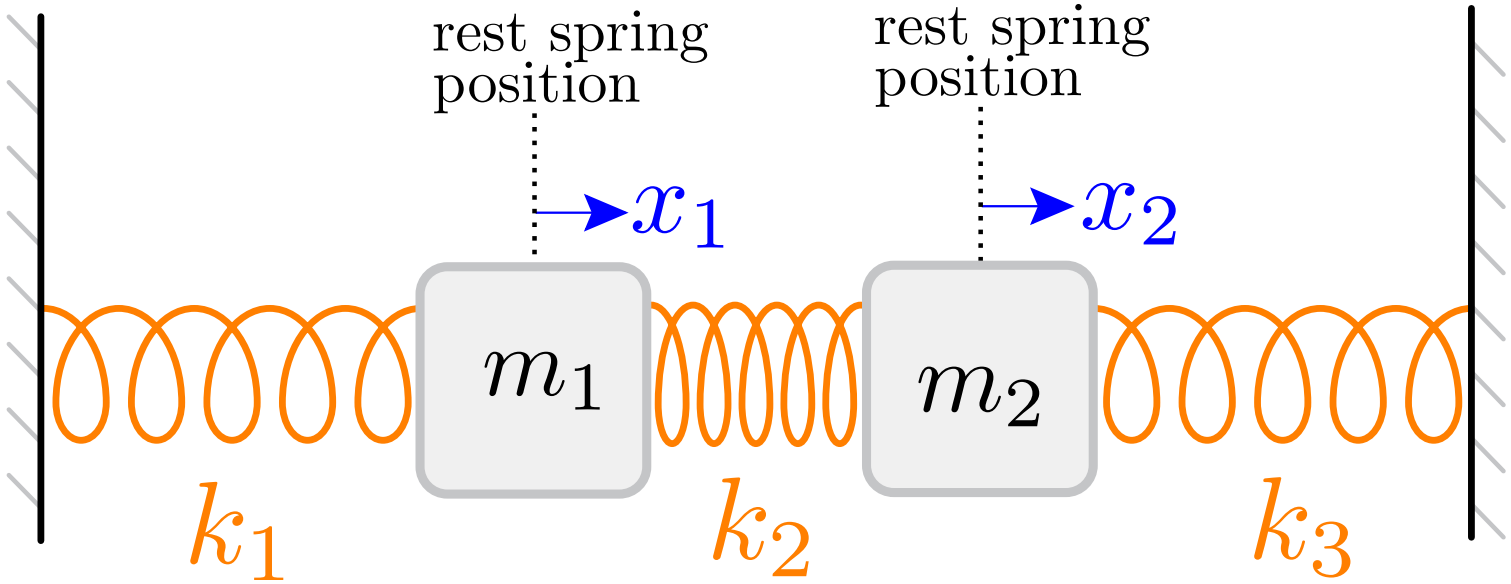
\includegraphics[width=0.5\textwidth]{documents/l7/springs.png}
\end{figure}

The displacements $x_1$ and $x_2$ satisfy two simultaneous second-order equations involving both variables. It turns out that we can eliminate $x_2$ to get a single fourth-order homogeneous ODE with constant coefficients for $x_1$.

For $k_1$ the compression or extension is given by $x_1$, for $k_2$ it is $x_2-x_1$, and for $k_3$ we have $-x_2$.

Using this we can then determine that the force on the first mass is: $m\ddot{x_1}=-k_1x_1+k_2(x_2-x_1)= -(k_1+k_2)x_1+k_2x_2$\\
And for the second mass we similarly have : $m\ddot{x_2}=-k_2(x_2-x_1)-k_3x_2=k_2x_1-(k_3+k_2)x_2$

Both equation form what's known as a \red{coupled system} of differential equation:\\
\centerline{$\begin{cases}
            m\ddot{x_1}= -(k_1+k_2)x_1+k_2x_2 \\
            m\ddot{x_2}=k_2x_1-(k_3+k_2)x_2
        \end{cases}$}

These two equations together are a system of two second-order linear differential equations, each with two dependent
variables $x_1$ and $x_2$ The approach we will take for now is to eliminate one of the dependent variables to obtain a single equation involving only the other dependent variable.

Notice that we can write $x_2$ in terms of $x_1$ and $\ddot{x_1}$ using the first DE: $x_2=\frac{m_1}{k_1}\ddot{x_1}+\frac{k1+k2}{k2}x_1$

Plugging this into the second equation and reducing, we get a 4th-order differential equation:\\
\centerline{\large$\boxed{m_1m_2x_1^{(4)}+\big(m_2(k_1+k_2)+m_1(k_2+k_3)\big)\ddot{x_1}+\big(k_1k_2+k_1k_3+k_2k_3\big)x_1=0}$}

This is a fourth-order homogeneous constant coefficient ODE for $x_1$.\\
To solve these higher-order ODEs we'll have to use the characteristic polynomial, the same way we did in second-order ODEs.
However for an $n$-th order linear ODE, we need $n$ linearly independent solutions, and linear independence of $n$ functions is a much more sophisticated notion than the linear independence of $2$ functions.

\subsection{Span of a set of functions}

\begin{dent}{Definition :}
    Suppose that $f_1,...,f_n$ are functions. The \red{span} of $f_1,...,f_n$ is the set of \red{all linear combination} of $f_1,...,f_2$:\\
    \centerline{\large$\boxed{\operatorname{Span}(f_1,..,f_n)=\bigl\{\text{all functions }c_1f_1+...+c_nf_n,\ \text{with } c_1,...,c_n\in \R \bigr\}}$}\vspace{-25pt}

    \begin{dent}{}

        Note: sometimes we allow the numbers $c_1,...,c_n$ to be \red{complex} and sometimes we allow them to be only \red{real}.\\
        The span of a set of functions is always a \red{vector space}.
    \end{dent}

\end{dent}

\newgeometry{width=18.625cm, bottom=2cm, top=2cm}

\subsection{Vector Spaces}

\begin{dent}{Example :}
    The 2-dimensional $(x,y)$-plane is a vector space. The vectors are the ordered pairs $(x,y)$ that add component-wise: $(x_1,y_1)+(x_2,y_2)=(x_1+x_2,y_1+y_2)$ There is a zero element and you can scale vectors by real numbers: $a(x,y)=(ax,ay)$
\end{dent}

\begin{dent}{Definition :}
    Suppose that $S$ is a set of elements called \red{vectors} equipped with two laws: a law for adding vectors in $S$, called \red{vector addition}, and a law for multiplying vectors in $S$ by real numbers, called \red{scalar multiplication}. Then $S$ is a \red{real vector space} if \red{all} the following are true:\\
    \begin{items}{-22pt}{-35pt}
        \item There is a \red{zero vector} in $S$: a vector $0$ in $S$ such that $v+0=v$ for every vector $v$ in $S$.
        \item Multiplying any one vector in $S$ by a real number gives another vector in $S$: if $v$ is in $S$ and $a$ is a real number, then $av$ is in $S$ too.
        \item Adding any two vectors in $S$ gives another vector in $S$: if $v$ and $w$ are in $S$, then the vector $v+w$ is in $S$.
    \end{items}
    \begin{dent}{}

        Note: This definition can also be used to define a \red{complex vector space}; it's the same thing as a real vector space, but scalar multiplication is defined for complex numbers instead of just real numbers.
    \end{dent}
\end{dent}

\begin{dent}{Example :}
    The set of all real-valued functions forms a real vector space. The constant $0$-function is the zero vector. Vector addition is addition of functions point-wise $(f+g)(x)=f(x)+g(x)$. Scalar multiplication is multiplying a function by a real number at each point, $af(x)=(a)(f(x))$.
\end{dent}

\begin{dent}{Counter-example :} The set of all non-negative functions is not a real vector space because $x^2$ is in this set, but $(-1)(x^2)=-x^2$ is not.
\end{dent}

\begin{dent}{Counter-example :}
    The set containing only the $x$- and $y$-axis is not a vector space because if we add two nonzero elements we don't always stay in the space, $(1,0)+(0,1)=(1,1)$ is not on either axis.
\end{dent}

\begin{dent}{Theorem :}
    \red{The set of all homogeneous solutions to a linear ODE is a vector space.}
\end{dent}

\subsection{Linear Independence}

\begin{dent}{Definition :}
    Vectors $v_1,...,v_n$ are \red{linearly dependent} (think redundant) if at least one of them is a linear combination of the others. Otherwise, call them \red{linearly independent}.
\end{dent}

\begin{dent}{Example :}
    In a vector space consisting of functions, each function is a vector. The functions $e^{2t}$, $e^{-3t}$ are \red{linearly independent}.
\end{dent}\vspace{-35pt}

\begin{dent}{}

    Note: For a set of 2 vectors, the definition of linear dependence and linear independence reduces to what we have learned
    before $v_1$ and $v_2$ are linearly dependent if one is a scalar multiple of the other. Otherwise, they are linearly independent.
\end{dent}

\begin{dent}{Example :}
    The functions $f_1=e^{2t}$, $f_2=e^{-3t}$, $f_3=e^{2t}+e^{-3t}$ are linearly \red{dependent}. The third function is a linear combination of the first two: $f_3=f_1+f_2$

    Each function is a linear combination of the other two: $f_1=f_3-f_2$ and similarly $f_2=f_3-f_1$
\end{dent}

\begin{dent}{Equivalent definition :}
    Vectors $v_1,...,v_n$ are \red{linearly dependent} if there exist numbers $c_1,...,c_n$ \red{not all zero} such that $c_1v_1+...+c_nv_n=0$.

    In the previous example we found that $f_1=f_3-f_2$, $f_2=f_3-f_1$, and $f_3=f_1+f_2$\\
    Symmetrically this can be written as $f_1+f_2-f_3=0$
\end{dent}

\begin{dent}{Example :}
    The three functions $e^{2t}$, $e^{-3t}$, $5e^{2t}+7e^{-3t}$ are linearly \red{dependent}, because:\\
    \centerline{$(-5)e^{2t}+(-7)e^{-3t}+(-1)\big(5e^{2t}+7e^{-3t}\big)$}

    The meaning of linear dependence is that at least one of the functions on the list is redundant (and can be expressed as a linear combination of the others.)
\end{dent}

\subsection{A Basis}

\begin{dent}{Definition :}
    A basis of a vector space $S$ is a list of vectors $v_1,...,v_n$ such that:
    \begin{items}{-10pt}{-10pt}
        \item $\operatorname{Span}(v_1,...,v_n)=S$
        \item The vectors $v_1,...,v_n$ are linearly \red{independent}.
    \end{items}
\end{dent}

\begin{dent}{Example :}
    The vectors $(1,0,0)$, $(0,1,0)$, $(0,0,1)$ form a basis for $\R^3$. This is because any vector $(x,y,z)$ can be written as a linear combination of these 3 basis vectors, and these 3 basis vectors are linearly independent:
    $c_1(1,0,0)+c_2(0,1,0)+c_3(0,0,1)=(0,0,0)$ \red{only} if $c_1$, $c_2$, $c_3$ all equal zero.
\end{dent}

The vector spaces that are relevant to differential equations are vector spaces of functions. A basis of a vector space of
functions is given as a list of functions $f_1,...,f_n$. Think of the functions in the basis as "basic building block".\\
By definition, every function in $S$ can be built from $f_1,...,f_n$. And there is no redundancy in the list, no
building block could have been built from the others.

The vector space of solutions to a homogeneous ODE consists of infinitely many functions. To describe it compactly,
we give a \red{basis} of the vector space. For a second-order linear homogeneous differential equation, the basis has only 2 functions.

\begin{dent}{Note :} A vector space has many different bases.

    The vectors $(1,0)$ and $(0,1)$ form a basis for $\R^2$, but so do any other pair of linearly independent vectors, such as $(1,0)$ and $(1,1)$.

    The space of solutions to $\ddot{y}+y=0$ is spanned both by the basis $e^{it}$, $e^{-it}$ and the basis $\cos(t)$, $\sin(t)$.
    \linecenter{(Here, we allow complex linear combinations of the basis functions.)}
\end{dent}

\subsection{Dimensions}

It turns out that although a vector space can have different bases, each basis has \red{the same number of vectors} in it.
\begin{dent}{Definition :}
    The \red{dimension} of a vector space is the number of vectors in \red{any} basis.
\end{dent}

\begin{dent}{Example :}
    The vector space $\R^3$ is a $3$-dimensional real vector space, since there are $3$ vectors in the basis : $(1,0,0)$, $(0,1,0)$, $(0,0,1)$

    The space of solutions to the homogeneous equation $\ddot{y}+\dot{y}-6y=0$ is $2$-dimensional, since the basis $e^{2t}$, $e^{-3t}$ has $2$ elements.
\end{dent}

In the examples involving differential equations above, the dimension equals the order of the homogeneous linear ODE.\\
It turns out that this holds in general.
\begin{dent}{Dimension Theorem :} \red{The dimension of the space of solutions to an $n$\color{red}-th order homogeneous ODE with constant coefficients is }$n$
\end{dent}

In other words, the number of parameters needed in the general solution to an $n$-th order homogeneous ODE with constant
coefficients is $n$.

\newpage

\subsection{Higher order linear ordinary differential equations}

Given $a_ny^{(n)}+...+a_1\dot{y}+a_0y=0$ we can apply the method seen with second-order linear homogeneous differential equations to higher-order differential equations.

Starting with the characteristic equation: $a_nr^n+...+a_1r+a_0=0$ we then proceed to factor the polynomial with respect to its roots: \vspace{-2mm}
\linecenter{$\mathcal{P}(r)=a_n(r-r_1)(r-r_2)...(r-r_n)$}

As we can see there are guaranteed to be $n$ roots counted with multiplicity by the fundamental theorem of algebra. They can be distinct or repeated.\\
If $r,..,r_n$ are \red{distinct}, then the functions $e^{r_1t}, ...,e^{r_nt}$ form a basis for the vector space of solutions to the constant coefficient ODE. In other words, the constant general solution is:
\linecenter{$c_1e^{r_1t}+...+c_ne^{r_nt}$}

Complex roots always appear in pairs of conjugates, and if some of the roots are complex, the coefficients will have to be complex as well.

If $r_1,..,r_n$ are \red{not distinct}, then $e^{r_1t}, ...,e^{r_nt}$ cannot be a basis since some of these functions are linearly dependent (redundant). If a particular root is repeated $m$ times then we'll need to replace the copies by $e^{rt}, re^{rt}, ..., r^{m-1}e^{rt}$

\subsection{Complex and Real valued basis}

Let $y(t)$ be a complex-valued function of a real-valued variable $t$. If $y$ and $\overline{y}$ are part of a
basis of solutions to a homogeneous linear system of ODEs with real coefficients, then replacing $y,\overline{y}$ by $\Re\big(y\big),\Im\big(y\big)$ gives a new pair of homogeneous solutions.

This is true, because any solution is a linear combination of the old basis, and can be converted to a linear combination of the new list by substituting $y=\Re\big(y\big)+i\Im\big(y\big)$ and $\overline{y}=\Re\big(y\big)-i\Im\big(y\big)$.

This new list is linearly independent. If it isn't then substituting $\Re\big(y\big)=\frac{y+\overline{y}}{2}$ and $\Im\big(y\big)=\frac{y-\overline{y}}{2i}$ would show that the old basis is linearly dependent, which is impossible for a basis.

\subsection{Existence and uniqueness}

The existence and uniqueness theorem comes in handy if we want to know whether a single solution is a solution to the differential equation.

Let $\mathcal{P}_{n-1}(t),...,\mathcal{P}_0(t),q(t)$ be continuous functions on an open interval $I$. Let $a\in I$, and let $b_0,...,b_{n-1}$ be given numbers. Then there exists a unique solution on $I$ to the $n$-th order linear ODE:
\linecenter{$y^{(n)}+\mathcal{P}_{n-1}(t)y^{(n-1)}+...+\mathcal{P}_1(t)\dot{y}+\mathcal{P}_0(t)y=q(t)$}

This solution satisfies initial conditions $y(a)=b_0, \dot{y}(a)=b_1, ..., y^{(n-1)}(a)=b_{n-1}$.

As before, \red{existence} means that there is \red{at least} one solution; \red{uniqueness} means that there \red{is only} one solution.
The theorem says that, given an $n$-th order linear ODE, a single solution can be found by giving $n$ numbers, namely the values of $y(a),\dot{y}(a),...,y^{(n-1)}(a)$ as the initial conditions.

The existence and uniqueness theorem in the homogeneous case explains the dimension theorem we stated previously. Each solution $y(t)$ determines a set of initial conditions, given by:
\linecenter{$y(t)\to\Big(y(a),\dot{y}(a),...,y^{(n-1)}(a)\Big)$}

On the other hand, the existence and uniqueness theorem says that each set of initial conditions specifies exactly one solution. The sequence of numbers $\Big(y(a),\dot{y}(a),...,y^{(n-1)}(a)\Big)$ constitutes a vector in $\R^{n}$ and the 1-to-1 correspondence between solutions and sets of initial conditions given by existence and uniqueness theorem proves the dimension theorem.

\chapter{Exponential Response and Resonance}

\section{Operators and Exponential Response}

\subsection{Linear Operators}

In any linear homogeneous differential equation, we've seen that if $c_1y_1$ and $c_2y_2$ were solutions then $c_1y_1+c_2y_2$ was also a solution to the equation. This is known by using superposition, however, we'll see why this work using \red{linear operators}. These operators use an input function to return a different function.

The \red{differential operator} $\frac{d}{dt}$ takes an input function $y(t)$ and returns $\frac{dy}{dt}$, however, it can also be called $D$.\\ For instance : $De^{4t}=4e^{4t}$. Since this operator is linear this means that we have $D(f+g)=Df+Dg$ and $D(af)=aDf$.

Because of this, $D$ behaves well with respect to linear combinations, namely $D(c_1f_1,...,c_nf_n)=c_1Df_1+...+c_nDf_n$

\begin{dent}{Definition :}
    In general, a \red{linear operator} $L$ is any operator that satisfies $L(f+g)$ and $L(af)=aLf$
\end{dent}
\begin{dent}{Example :}
    The operator $L=D^2+p(t)D+q(t)$ is a linear operator since $D$ is linear and the linear combination of linear operators is once again a linear operator.
\end{dent}

To apply a product of two operators, apply each operator in succession. For instance, $DDy$ means take the derivative of $y$, and then take the derivative of the result; therefore we write $D^2y=\ddot{y}$.

To apply a sum of two operators, apply each operator to the function and add the results. For instance, $(D^2+D)y=D^2y+Dy=\ddot{y}+\dot{y}$

Any number can be viewed as the “multiply-by-the-number" operator: for instance, the operator $5$ transforms the function $\sin(t)$ into the function $5\sin(t)$. In particular, the “identity" operator $1$ is the operator: $1f=f$ for all functions $f$.

Similarly, we can multiply by any function of $t$, and this is also a linear operator. For instance, the operator $t^2$ transforms the function $\sin(t)$ into the function $t^2\sin(t)$.

\begin{dent}{Example :}
    The differential equation $2\ddot{y}+3\dot{y}+5y=0$ can be rewritten as $(2D^2+3D+5)y=0$ becoming $\P(D)y=0$
\end{dent}

\newpage

Using this notion we can study polynomial differential operators which have the form:
\linecenter{$\mathcal{P}(D)=a_nD^n+...+a_1D+a_0$}

All operators of this form are linear. In addition to being linear operators, they are also \red{time-invariant} operators, meaning that if $x(t)$ solves $\mathcal{P}(D)x=f(x)$, then $y(t)=x(t-t_0)$ solves $\mathcal{P}(D)y=f(t-t_0)$

This translates to: delaying the input signal $f(t)$ by $t_0$ seconds delays the output signal $x(t)$ by $t_0$ seconds.\\
If we know that $x(t)$ is a solution to $\mathcal{P}(D)x=f(t)$, we can solve $\mathcal{P}(D)y=f(t-t_0)$ by replacing $t$ by $t-t_0$ in $x(t)$.\\ This is a useful property because it gives us the solutions to many differential equations quickly.

A system that can be modeled using a linear time-invariant operator is called an \red{LTI} (\red{linear time-invariant}) system.

\begin{figure}[ht]
    \centering
    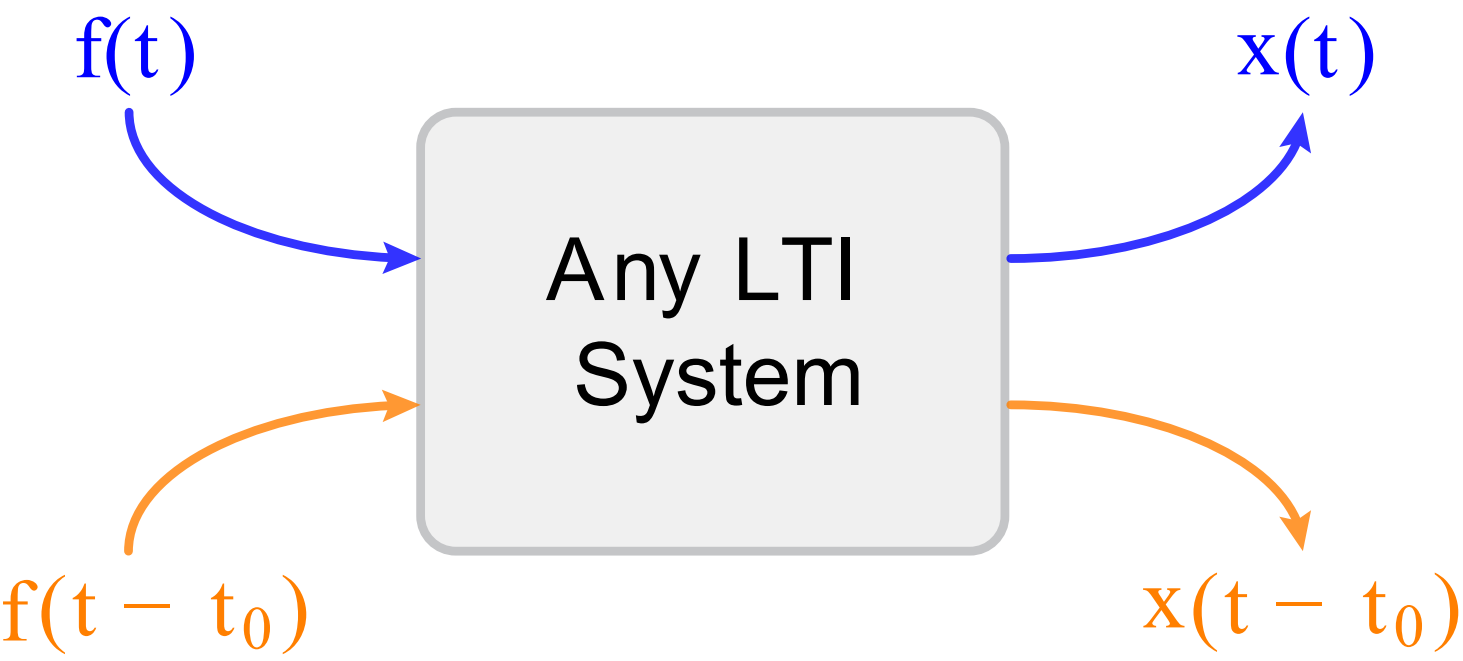
\includegraphics[width=0.35\textwidth]{documents/l8/LTI.png}
\end{figure}

\begin{dent}{Example :}
    Consider the differential equation $\dot{x}+x=\cos(t)$

    Variation of parameters or integrating factors will lead us to the general solution to this differential equation:
    \linecenter{$x(t) =\frac{1}{2}\cos(t)+\frac{1}{2}\sin(t)+c_1e^{-t}$}

    Now suppose that we want to solve the equation $\dot{x}+x=\sin(t)$. Since $\sin(t)=\cos(t-\frac{\pi}{2})$, time invariance will provide us with:
    \linecenter{$y(t) =\frac{1}{2}\sin(t)\frac{1}{2}\cos(t)+c_2e^{-t}$}

    This agrees with the solution we'd get if we had used a variation of parameters or integrating factors, but we found the solution effortlessly from the first.
\end{dent}

\subsection{Inhomogeneous Equation}

In \hyperlink{page.9}{\underline{Lesson II}} we've seen how to solve inhomogeneous differential equations using the superposition theorem:\\
\centerline{$y_{general}=y_{homogeneous}+y_{particular}$}

We'll now see with the previously seen notion why this is the case.

Let $L$ be the linear operator $L=\mathcal{P}_n(t)D^n+...+\mathcal{P}_1(t)D+\mathcal{P}_0(t)$ then the differential equations become:\vspace{-8pt}

\begin{figure}[ht]
    \renewcommand{\arraystretch}{1.5}
    {\setlength{\tabcolsep}{2em}
        \begin{tabular}{c l}
            inhomogeneous case & $Ly=q(t)$ \\
            homogeneous case   & $Ly=0$
        \end{tabular}}
\end{figure}

Let $y_p$ be a particular solution to the inhomogeneous equation $L(y_p)=q(t)$. Let $y_h$ be a homogeneous solution $L(y_h)=0$. Then $L(y_p+y_h)=q+0=q$

Letting $y$ be the solution to $Ly=q(t)$ we then have by linearity $L(y-yp)=0$.

Therefore $y-yp=y_h$ is a solution to the associated homogeneous equation. in other words $y=y_h+y_p$

\red{The result of this is the key point of linearity in the inhomogeneous case}. It lets us build \red{all} the solutions to an inhomogeneous DE out of one particular solution provided that you have already solved the associated homogeneous ODE.

\newpage

\subsection{Particular Solution}

\begin{dent}{Problem :}
    Let $r$ be any number. Then what would $\lr{2D^2+3D+5}e^{rt}$ look like?
\end{dent}
\begin{dent}{Solution :}
    Applying the chain rule we find $\lr{2D^2+3D+5}e^{rt}=\lr{2r^2+3r+5}e^{rt}$\\
    We can quickly notice $\P(D)=\P(r)$. This turns out to be true for all $r$

\end{dent}
\begin{dent}{Theorem :}
    \red{For any polynomial} $\P$ \red{and real number} $r$ \red{:} $\color{red}\P(D)e^{rt}=P(r)e^{rt}$
\end{dent}

Using this theorem we might be able to find a particular solution to a given differential equation, such as $P(D)y=e^{rt}$.\\
In this case we then have $\P(D)e^{rt}=\P(r)e^{rt}$ which quickly becomes $\P(D)\lr{\frac{e^{rt}}{\P(r)}}=e^{rt}$.

This is called the \red{Exponential Response Formula}, and as we can see $\frac{e^{rt}}{\P(r)}$ becomes a particular solution to the differential equation $\P(D)y=e^{rt}$ granted $\P(r)\neq 0$.

This remains nothing but a particular solution. To obtain the general solution to our equation we can use the superposition theorem after having found the homogeneous solution.

\subsection{Existence and Uniqueness}

The existence and uniqueness theorem says that $\P(D)y=e^{rt}$ should have a solution even if $\P(r)=0$.\\
Let's start with the one case: Suppose that $\P$ is a polynomial and $\P(r_0)=0$, but $\P'(r_0)\neq 0$ for some number $r_0$. Then:
\linecenter{$\ds{\boxed{x_p=\frac{1}{\P'(r_0)}te^{r_0t}\quad\textcolor{black}{\text{is a particular solution to}}\quad \P(D)x=e^{r_0t}}}$}

\begin{dent}{Proof :}
    We want to solve $\P(D)y=e^{r_0t}$ knowing that $\P(D)e^{rt}=\P(r)e^{rt}$. In other words $\P(D)e^{r_0t}=\P(r_0)e^{r_0t}$.\\
    The catch is that since $\P(r_0)=0$, we can not simply divide the left-hand side.

    Therefore we'll want to know what happens as $r$ approaches $r_0$ by differentiating with respect to $r$ and substituting $r$ for $r_0$:
    \linecenter{\large$\ds{\frac{\vard}{\vard r}\big(\P(D)e^{rt}\big)=\frac{\vard}{\vard r}\big(\P(r)e^{rt}\big)=\P'e^{rt}+\P(r)te^{rt}}$}

    However the left hand side becomes also $\ds{\frac{\vard}{\vard r}\big(\P(D)e^{rt}\big)=\P(D)\lr{\frac{\vard}{\vard r}e^{rt}}=\P(D)\big(te^{rt}\big)}$

    Thus as $r$ approaches $r_0$, $\P(r_0)=0$ and therefore we get $\P(D)\big(te^{r_0t}\big)=\P'(r_0)e^{r_0t}$.\\
    The important part here is that since $\P'(r_0)\neq 0$ we can divide it without causing any issues. Hence we obtain the following:
    \linecenter{\large$\ds{\boxed{\P(D)\lr{\frac{te^{r_0t}}{\P'(r_0)}}=e^{r_0t}}}$}

    The particular solution is then deduced as $\ds{y_p=\frac{te^{r_0t}}{\P'(r_0)}}$ for the equation $\P(D)y=e^{r_0t}$
\end{dent}

\begin{dent}{Example :}
    Find a particular solution to $\ddot{x}-4x=e^{-2t}$

    To do so, we find the characteristic equation as $\P(r)=r^2-4$, thus $\P(-2)=0$. But $\P'(-2)=-4$. Therefore we can apply the derivative form of the ERF, giving the particular solution:
    \linecenter{$\boxed{x_p=\frac{te^{-2t}}{-4}}$}
\end{dent}

In a generalised way if $\P$ is a polynomial and $r_0$ is an number such that $\P(r_0)=\P'(r_0)=...=\P^{(m-1)}(r_0)=0$ and $\P^{(m)}(r_0)\neq0$
then the particular solution to $\P(D)y=e^{r_0t}$ becomes:
\linecenter{$\boxed{y_p=\frac{1}{\P^{(m)}(r_0)}t^me^{r_0t}}$}



\begin{dent}{Example :}
    Solve the system $\ddot{x}+x=e^{it}$ with initial conditions $\dot{x}(0)=1$ and $x(0)=0$

    Utilizing the characteristic equation, we find the roots being $\pm i$. Since $i$ is the root of the characteristic polynomial then the exponential response formula incites us to find the smallest integer $s$ for which $\P^{(i)}\neq 0$. However since we have $\P'(r)=2r$, and by extension $\P'(i)=2i\neq 0$ then $s=1$ which leads us to the particular solution:
    \linecenter{\large{$x_p(t)=\frac{1}{\P'(i)}te^{it}=\frac{1}{2i}te^{it}$}}
    Which can be rewritten as:
    \linecenter{\large$\boxed{x_p(t)=\frac{1}{2}te^{it-i\frac{\pi}{2}}}$}

    The general solution is then simply:
    \linecenter{\large$x(t)=c_1e^{it}+c_2e^{-it}+\frac{1}{2}te^{it-i\frac{\pi}{2}}$}

    All that would be left to do is find constants satisfying initial conditions.

    The solution for this system results being:
    \linecenter{\large$\boxed{\frac{3}{4}e^{it}+\frac{1}{4}e^{-it}+\frac{1}{2}te^{it-i\frac{\pi}{2}}}$}
\end{dent}

\subsection{Basis of a Higher Order System}

Using operators we can look closer at the method used to find a basis of solutions to a constant-coefficient homogeneous ODE written as $\P(D)y=0$.

Consider the following differential equation $y'''-10y''+32y'-30y=0$\\
Rewriting this using operator notation we get $\P(D)y=0$, where $\P(r)=r^3-10r^2+32r-30$ is the characteristic polynomial. By factoring this polynomial we find $\P(r)=(r-2)(r-3)(r-5)$. Since the order of this polynomial is $3$ then the dimension of the vector space of solutions is also $3$.\vspace{-25pt}

\begin{dent}{}

    \centering$e^{2t}$ is a solution since $\P(D)e^{2t}=\P(2)e^{2t}=0$\\
    $e^{3t}$ is a solution since $\P(D)e^{3t}=\P(3)e^{3t}=0$\\
    $e^{5t}$ is a solution since $\P(D)e^{5t}=\P(5)e^{5t}=0$
\end{dent}
However simply because there are $3$ solutions does not mean that they form a basis, for this to be true, all terms should be linearly independent.
We would need to see if $e^{5t}=c_1e^{2t}+c_2e^{3t}$ for some constants $c_1$ and $c_2$.

One way to see that this is impossible is to apply $(D-2)(D-3)$ to both sides which would give:
\begin{eq}{-5pt}{-30pt}
    \blu(D-2)(D-3)e^{5t}&\blu=(D-2)(D-3)\big(c_1e^{2t}+c_2e^{3t}\big)\\
    &\blu=c_1(D-2)(D-3)e^{2t}+c_2(D-2)(D-3)e^{3t}\\
    &\blu=c_1\cdot0+c_2\cdot0=0
\end{eq}

And the left hand side simply becomes $(D-2)(D-3)e^{5t}=(5-2)(5-3)e^{5t}\neq0$.
As such this implies that $e^{5t}$ is not a linear combination of $e^{2t}$ and $e^{3t}$. Therefore since $e^{2t}$,$e^{3t}$,$e^{5t}$ are linearly independent, they form a basis for a $3$-dimensional space.

\newpage

\subsection{Repeated Roots}

It's rare to encounter a higher-order differential equation with repeated roots, however, they can be encountered, in which case it is important to know how to deal with them.

\begin{dent}{Example :}
    Find a basis of solutions to $D^3y=0$ (roots $0$,$0$,$0$)

    Integrating three times we get the following solution:\\
    \centerline{$y=c_1t^2+c_2t+c_3$}
    Since $t^2$, $t$, and $1$ are linearly independent, they form a basis for the space of solutions.

\end{dent}

\begin{dent}{Example :}
    Find a basis of solutions to $(D-5)^3y=0$

    Since the characteristic polynomial is $(r-5)^3$, and has roots $5$, $5$, $5$ we might hope that $e^{5t}$, $te^{5t}$, $t^2e^{5t}$ are a basis. However, we need to know why this is the case.

    We know that $D-5$ sends $e^{5t}$ to $0$, so what does $D-5$ do to $u(t)e^{5t}$?
    \begin{eq}{-5pt}{-30pt}
        \blu (D-5)u(t)e^{5t}&\blu=(\dot{u}e^{5t}+5ue^{5t})-5ue^{5t}\\
        &\blu=\dot{u}e^{5t}
    \end{eq}

    Replacing $(D-5)$ by $(D-5)^2$ and $(D-5)^3$ on the left we get the following:
    \begin{eq}{-5pt}{-30pt}
        \blu(D-5)^2ue^{5t}&\blu=\ddot{u}e^{5t}\\
        \blu(D-5)^3ue^{5t}&\blu=u^{(3)}e^{5t}
    \end{eq}

    Therefore in order for $ue^{5t}$ to be a solution to $(D-5)^3y=0$ the function $u^{(3)}$ must be $0$, meaning that $u=a+bt+ct^2$. We then have as expected:
    \linecenter{$ue^{5t}=ae^{5t}+bte^{5t}+ct^2e^{5t}$}
    Since $t^2$, $t$, $1$ are linearly independent functions, so are $e^{5t}$, $te^{5t}$, $t^2e^{5t}$. Thus $e^{5t}$, $te^{5t}$, $t^2e^{5t}$ form a basis.

    If a characteristic polynomial $\P(r)$ has a root $r$ that is repeated $k$ times, then $e^{rt}$, $te^{rt}$, $t^2e^{rt}$, ..., $t^{k-1}e^{rt}$ are independent solutions to the differential equation $\P(D)y=0$
\end{dent}

\subsection{Summing Up}

\begin{dent}{Example :}
    Find the general solution to the differential equation $2\ddot{x}+\dot{x}+x=1+2e^{t}$

    Since this is an inhomogeneous linear equation, the general solution has the form $x_p+x_h$. The characteristic polynomial is $^\P(s)=2s^2+s+1$ with roots $\frac{(-1\pm\sqrt{7}i)}{4}$, so the general homogeneous solution is given by:
    \begin{eq}{-10pt}{-25pt}
        \blu x_h(t)&\blu=e^{-t/4}\Big(c_1\cos\big(\frac{\sqrt{7}t}{4}\big)+c_2\sin\big(\frac{\sqrt{7}t}{4}\big)\Big)\\
        &\blu=Ae^{-t/4}\cos\big(\frac{\sqrt{7}t}{4}-\phi\big)
    \end{eq}

    Since the input signal is a linear combination of $1$ and $2e^t$ we'll have to find particular solutions $x_1$ to $\P(D)x=1$ and $x_2$ to $\P(D)x=2e^t$ and apply the superposition principle to find our general solution.

    The constant function $1$ is an exponential $e^{0t}$, meaning that $\P(D)x=1$ has a particular solution:
    \linecenter{$\ds{x_1=\frac{1}{\P(0)}=1}$}
    Similarly, we can solve for $x_2$:
    \linecenter{$\ds{x_2=\frac{1}{\P(1)}2e^t=\frac{1}{2}e^t}$}
    We've then found the particular solution to $\P(D)x=1+e^t$ by superposition of $x_1$ and $x_2$ as $x_p=1+\frac{1}{2}e^t$.

    This then allows us to find the general solution to our differential equation:
    \large\linecenter{$\boxed{\ds{x(t)=1+\frac{1}{2}e^t+Ae^{-t/4}\cos\Big(\frac{\sqrt{7}t}{4}-\phi\Big)}}$}

\end{dent}

\newpage

\section{Complex Replacement Gain and Phase Lag Stability}

\subsection{Complex Replacement}

Suppose we are studying the tides in a harbor. Let $x$ be the water level of the harbor and $y$ the water level of the ocean. The input signal is $y$, which is responsible for the changing tides $x$ in the harbor, the system response.

Assuming that the ocean and the harbor are connected by a narrow channel, the flow will be slow and not turbulent. This allows us to assume that the flow rate is pressure-driven, and is linearly proportional to the pressure difference. Furthermore, the pressure difference is linearly proportional to the difference in water level between the ocean and the harbor.


We'll be trying to model the rising and falling tides with an appropriate differential equation.

Since we'll be expecting an oscillating input we'll have to come acquainted with \red{complex replacement}. A method for finding solutions to an inhomogeneous linear differential equation with oscillating input:
\linecenter{$\ds{\P(D)x=\cos(\omega t)}$}

To solve these particular equations we can start by complexifying the input signal as $\Re(e^{i\omega t})$
or complexify the entire differential eqaution as $\P(D)z=e^{i\omega t}$.

Using the exponential response formula we can then find a complex particular solution:
\linecenter{$z_p=\ds{\frac{e^{i\omega t}}{\P(i\omega)}}$}

The particular solution of the original differential equation is then obtained by taking the real part of the complex particular solution, $x_p=\Re(z_p)$.

\begin{dent}{Proof :}
    If $z=x_1+ix_2$ is a solution to the complex replacement differential equation $\P(D)z=e^{i\omega t}$.\\
    Then since $\P$ has real coefficients, taking the real parts of both sides gives $\P(D)x_1=\cos(\omega t)$.

    This means that $x_1$ is a solution to the original differential equation.
\end{dent}

\begin{dent}{Example :}
    Find a solution to $\ddot{x}+4x=\cos(2t)$

    Replacing $\cos(2t)$ by $\Re(e^{2it})$ and complexifying the differential equation as $\ddot{z}+4z=e^{2it}$ we can find the characteristic polynomial $\P(r)=r^2+4$ and $\P(2i)=0$, which means we need to use the derivative of the exponential response formula $\P'(r)=2r$.\\
    The particular solution then becomes:
    \linecenter{$\ds{z_p=\frac{te^{2it}}{\P'(2i)}=\frac{te^{2it}}{4i}}$}

    Taking the real part of this solution we find $x_p=\frac{t}{4}\sin(2t)$

\end{dent}

\subsection{Phase Lag}

We want to show how the amplitude and phase lag of the system response depends on the system parameters and the input frequency. To do so, we will use the complex replacement and introduce \red{complex gain}.

Let's state the general picture for reference. We have an LTI system modeled by the differential equation $\P(D)x=\mathcal{Q}(D)y$ with $y$ input signal and $x$ system response.\\
The ERF and complex replacement tell us that if $y=\cos(\omega t)$, then a particular solution is given by
\linecenter{$x_p=\Re\big(G(\omega)e^{i\omega t}\big)$\hspace{1.25cm}where $G(\omega)=\frac{\mathcal{Q}(i\omega)}{\P(i\omega)}$ if $\P(i\omega)\neq0$}

\newpage

\begin{dent}{Going Further}
    The complexified equation is $\P(D)z=\Q(D)e^{i\omega t}$. If $\P(i\omega)\neq0$, the ERF gives us a particular solution of the form: $\ds{z_p=\frac{\Q(i\omega)}{\P(i\omega)}e^{i\omega t}}$.

    We can express this as $z_p=G(\omega)e^{i\omega t}$ or alternatively in polar form with $G(\omega)=|G(\omega)|e^{-i\phi}$ as $z_p=|G(\omega)|e^{i(\omega t-\phi)}$.

    The solution then becomes $x_p=|G(\omega)|\cos(\omega t-\phi)$

\end{dent}

\subsection{Tides}

Recall that we model the ocean tide by $\cos(\omega t)$, used as the input signal. The system response $x$ is the height of the water in the harbor.

Using the method of complex replacement to solve the differential equation we have $\dot{z}+kz=ke^{i\omega t}$ with input signal $e^{i\omega t}$

One particular solution determined by the ERF is $\ds{z_p=\frac{\Q(i\omega)}{\P(i\omega)}e^{i\omega t}=\frac{k}{i\omega + k}e^{i\omega t}}$

This shows that the system response to a complex exponential input signal is a \red{constant multiple} of that input signal. That constant is called the \red{complex gain}.
\linecenter{$G(\omega)=\frac{\text{complexified system repsonse}}{\text{complex system input}}$}

In our case the complex gain is $G(\omega)=\frac{k}{i\omega + k}$.\\
This complex number $G$ expressed as a ratio of two functions of time is \red{constant}. It depends upon the system parameters, but we regard them as fixed. We are interested in how it varies with the input angular frequency $w$ and write $G(X)$

\end{document}